\documentclass[11pt]{article}
\usepackage[margin=1in]{geometry}
\usepackage{setspace}\onehalfspacing
\usepackage{amsmath,amssymb}
\usepackage{graphicx,float}
\usepackage{booktabs,threeparttable}
\usepackage[authoryear,round]{natbib}
\usepackage[hidelinks]{hyperref}
\usepackage{caption}
\captionsetup{font=small,labelfont=bf}
\usepackage{enumitem}
\setlist{itemsep=2pt,topsep=4pt}
\usepackage{appendix}
\usepackage{xcolor}
\usepackage{array}
\usepackage[section]{placeins}
\newcolumntype{L}[1]{>{\raggedright\arraybackslash}p{#1}}
\newcommand{\authornote}[1]{\textcolor{red}{[AUTHOR: #1]}}
% generated by code/40_paper.py -- do not edit
\newcommand{\accChanges}{55}
\newcommand{\accForecast}{84}
\newcommand{\accNaive}{79}
\newcommand{\accWorsenings}{54}
\newcommand{\aidAllFourCurPool}{27}
\newcommand{\aidAllFourCurPoolCi}{\textminus{}1 to 62}
\newcommand{\aidAllFourCurWithin}{4}
\newcommand{\aidAllFourCurWithinCi}{\textminus{}13 to 23}
\newcommand{\aidAllFourFcPool}{76}
\newcommand{\aidAllFourFcPoolCi}{44 to 115}
\newcommand{\aidAllFourFcWithin}{4}
\newcommand{\aidAllFourFcWithinCi}{\textminus{}11 to 22}
\newcommand{\aidAllThreeCurPool}{11}
\newcommand{\aidAllThreeCurPoolCi}{\textminus{}2 to 26}
\newcommand{\aidAllThreeCurWithin}{\textminus{}1}
\newcommand{\aidAllThreeCurWithinCi}{\textminus{}8 to 7}
\newcommand{\aidAllThreeFcPool}{26}
\newcommand{\aidAllThreeFcPoolCi}{9 to 46}
\newcommand{\aidAllThreeFcWithin}{10}
\newcommand{\aidAllThreeFcWithinCi}{3 to 19}
\newcommand{\aidFoodFourCurPool}{38}
\newcommand{\aidFoodFourCurPoolCi}{\textminus{}1 to 94}
\newcommand{\aidFoodFourCurWithin}{7}
\newcommand{\aidFoodFourCurWithinCi}{\textminus{}17 to 38}
\newcommand{\aidFoodFourFcPool}{118}
\newcommand{\aidFoodFourFcPoolCi}{67 to 184}
\newcommand{\aidFoodFourFcWithin}{4}
\newcommand{\aidFoodFourFcWithinCi}{\textminus{}21 to 38}
\newcommand{\aidFoodThreeCurPool}{20}
\newcommand{\aidFoodThreeCurPoolCi}{1 to 43}
\newcommand{\aidFoodThreeCurWithin}{\textminus{}2}
\newcommand{\aidFoodThreeCurWithinCi}{\textminus{}14 to 12}
\newcommand{\aidFoodThreeFcPool}{45}
\newcommand{\aidFoodThreeFcPoolCi}{15 to 82}
\newcommand{\aidFoodThreeFcWithin}{25}
\newcommand{\aidFoodThreeFcWithinCi}{5 to 48}
\newcommand{\amnAnyDiag}{35}
\newcommand{\amnAnyN}{1,427}
\newcommand{\amnDerCorr}{0.20}
\newcommand{\amnDerCountries}{8}
\newcommand{\amnDerN}{902}
\newcommand{\amnExpAgree}{42}
\newcommand{\amnExpCorr}{0.13}
\newcommand{\amnExpN}{600}
\newcommand{\aucEvents}{1,009}
\newcommand{\aucN}{12,776}
\newcommand{\aucRaw}{0.79}
\newcommand{\aucRawFews}{0.85}
\newcommand{\aucRawFewsPct}{85}
\newcommand{\aucRawIPC}{0.84}
\newcommand{\aucRawIPCFews}{0.86}
\newcommand{\aucRawPct}{79}
\newcommand{\bcBetaFive}{22}
\newcommand{\bcBetaFour}{10}
\newcommand{\bcBetaOne}{10}
\newcommand{\bcBetaThree}{28}
\newcommand{\bcBetaTwo}{11}
\newcommand{\bcBudget}{45}
\newcommand{\bcBudgetHigh}{65}
\newcommand{\bcBudgetLow}{35}
\newcommand{\bcCostCrisisFive}{14}
\newcommand{\bcCostCrisisFour}{22}
\newcommand{\bcCostFiveCons}{1,200}
\newcommand{\bcCostFiveMid}{570}
\newcommand{\bcCostFiveUp}{350}
\newcommand{\bcCostFourCons}{1,900}
\newcommand{\bcCostFourMid}{920}
\newcommand{\bcCostFourUp}{560}
\newcommand{\bcCostOneCons}{150,000}
\newcommand{\bcCostOneMid}{99,000}
\newcommand{\bcCostOneUp}{87,000}
\newcommand{\bcCostThreeCons}{110,000}
\newcommand{\bcCostThreeMid}{84,000}
\newcommand{\bcCostThreeUp}{120,000}
\newcommand{\bcCostTwoCons}{100,000}
\newcommand{\bcCostTwoMid}{60,000}
\newcommand{\bcCostTwoUp}{46,000}
\newcommand{\bcCrisisFive}{3.2}
\newcommand{\bcCrisisFour}{2.0}
\newcommand{\bcCrisisOne}{0.0}
\newcommand{\bcCrisisThree}{0.0}
\newcommand{\bcCrisisTwo}{0.0}
\newcommand{\bcDeathsFiveCons}{37,600}
\newcommand{\bcDeathsFiveMid}{78,300}
\newcommand{\bcDeathsFiveUp}{127,300}
\newcommand{\bcDeathsFourCons}{23,500}
\newcommand{\bcDeathsFourMid}{49,100}
\newcommand{\bcDeathsFourUp}{80,000}
\newcommand{\bcDeathsOneCons}{300}
\newcommand{\bcDeathsOneMid}{500}
\newcommand{\bcDeathsOneUp}{500}
\newcommand{\bcDeathsThreeCons}{400}
\newcommand{\bcDeathsThreeMid}{500}
\newcommand{\bcDeathsThreeUp}{400}
\newcommand{\bcDeathsTwoCons}{400}
\newcommand{\bcDeathsTwoMid}{800}
\newcommand{\bcDeathsTwoUp}{1,000}
\newcommand{\bcDistinctHi}{150,000}
\newcommand{\bcDistinctLo}{46,000}
\newcommand{\bcFlaggedAreas}{3,376}
\newcommand{\bcFlaggedRounds}{11,671}
\newcommand{\bcGrossCons}{80}
\newcommand{\bcGrossCrisis}{6.5}
\newcommand{\bcGrossMid}{168}
\newcommand{\bcGrossUp}{274}
\newcommand{\bcOneHi}{n.a.}
\newcommand{\bcOneLo}{n.a.}
\newcommand{\bcOneShareFood}{\textminus{}4.4}
\newcommand{\bcPeople}{28}
\newcommand{\bcPhaseThree}{42}
\newcommand{\bcPhaseTwo}{50}
\newcommand{\bcSfourEmerg}{25}
\newcommand{\bcShareFive}{47}
\newcommand{\bcShareFour}{29}
\newcommand{\bcShareOne}{0.3}
\newcommand{\bcShareThree}{0.3}
\newcommand{\bcShareTwo}{0.4}
\newcommand{\bcSthreeCrisis}{34}
\newcommand{\bcSthreeEmerg}{60}
\newcommand{\bcSthreeStressed}{10}
\newcommand{\bcWastingHi}{14,000}
\newcommand{\bcWastingLo}{9,000}
\newcommand{\bcWholeHi}{1,900}
\newcommand{\bcWholeHiBudgetHi}{2,800}
\newcommand{\bcWholeLo}{350}
\newcommand{\bcWholeLoBudgetLo}{270}
\newcommand{\bootOffAllFews}{0.003}
\newcommand{\bootOffAllProj}{0.014}
\newcommand{\bootOffNewFews}{0.006}
\newcommand{\bootOffNewProj}{0.006}
\newcommand{\calCdrHi}{0.25}
\newcommand{\calCdrLo}{0.07}
\newcommand{\calCdrMid}{0.15}
\newcommand{\calFamHi}{1.9}
\newcommand{\calFamLo}{0.9}
\newcommand{\calFamMid}{1.5}
\newcommand{\calGamHi}{2.5}
\newcommand{\calGamLo}{0.6}
\newcommand{\calGamMid}{1.5}
\newcommand{\caseEtAreas}{678}
\newcommand{\caseEtCurFour}{9}
\newcommand{\caseEtCurThree}{173}
\newcommand{\caseEtFcFour}{26}
\newcommand{\caseEtFlagShare}{15}
\newcommand{\caseEtFlags}{103}
\newcommand{\caseEtNextFour}{24}
\newcommand{\caseEtNextThree}{162}
\newcommand{\caseEtRain}{\textminus{}1.1}
\newcommand{\caseSoAreas}{199}
\newcommand{\caseSoCurFour}{16}
\newcommand{\caseSoCurThree}{60}
\newcommand{\caseSoFcFour}{26}
\newcommand{\caseSoFlagShare}{48}
\newcommand{\caseSoFlags}{95}
\newcommand{\caseSoNextFour}{29}
\newcommand{\caseSoNextThree}{122}
\newcommand{\caseSoRain}{\textminus{}0.8}
\newcommand{\cgBarPerDeath}{4,000}
\newcommand{\cgBudgetHi}{86}
\newcommand{\cgBudgetLo}{28}
\newcommand{\cgFiftyHi}{120}
\newcommand{\cgFiftyLo}{36}
\newcommand{\cgFortyHi}{87}
\newcommand{\cgFortyLo}{26}
\newcommand{\cgHungerHi}{28}
\newcommand{\cgHungerLo}{4}
\newcommand{\cgThirtyHi}{65}
\newcommand{\cgThirtyLo}{20}
\newcommand{\cgWholeHi}{11,000}
\newcommand{\cgWholeLo}{2,100}
\newcommand{\chCountries}{18}
\newcommand{\chFcsCorr}{0.33}
\newcommand{\chHhsCorr}{0.34}
\newcommand{\chLcsCorr}{0.15}
\newcommand{\chN}{2,805}
\newcommand{\chRcsiCorr}{0.04}
\newcommand{\contribRawCur}{0.13}
\newcommand{\contribRawCurSe}{0.02}
\newcommand{\contribRawFc}{0.13}
\newcommand{\contribRawFcSe}{0.02}
\newcommand{\contribRawIPCCur}{0.12}
\newcommand{\contribRawIPCCurSe}{0.02}
\newcommand{\contribRawIPCFc}{0.08}
\newcommand{\contribRawIPCFcSe}{0.02}
\newcommand{\covCountries}{70}
\newcommand{\covPfour}{82}
\newcommand{\covPost}{0.002}
\newcommand{\covPostSe}{0.006}
\newcommand{\covPre}{\textminus{}0.010}
\newcommand{\covPrePhase}{0.130}
\newcommand{\covPrePhaseSe}{0.054}
\newcommand{\covPreSe}{0.019}
\newcommand{\covPthree}{69}
\newcommand{\csAreaMonths}{209,404}
\newcommand{\csAreas}{16,684}
\newcommand{\csCountries}{37}
\newcommand{\dCostBudgetHi}{220,000}
\newcommand{\dCostBudgetLo}{36,000}
\newcommand{\dCostCrisisHi}{2,700}
\newcommand{\dCostCrisisLo}{1,600}
\newcommand{\dCostEmergHi}{1,100}
\newcommand{\dCostEmergLo}{400}
\newcommand{\dCostWastHi}{910,000}
\newcommand{\dCostWastLo}{190,000}
\newcommand{\dCostWastMax}{2,800,000}
\newcommand{\dCostWastMin}{120,000}
\newcommand{\dCrisisHi}{28,000}
\newcommand{\dCrisisLo}{17,000}
\newcommand{\dDeathsHi}{970}
\newcommand{\dDeathsLo}{290}
\newcommand{\dEmergHi}{110,000}
\newcommand{\dEmergLo}{41,000}
\newcommand{\dShareHi}{0.4}
\newcommand{\dShareLo}{0.3}
\newcommand{\dWastHi}{240}
\newcommand{\dWastLo}{50}
\newcommand{\envBeta}{28}
\newcommand{\envPmHi}{9.6}
\newcommand{\envPmLo}{4.2}
\newcommand{\envShareIpc}{7}
\newcommand{\envSharePosRaw}{16}
\newcommand{\envShareRaw}{9}
\newcommand{\envUsdHi}{370}
\newcommand{\envUsdLo}{274}
\newcommand{\famCame}{0}
\newcommand{\famEpisodes}{5}
\newcommand{\famFlag}{50}
\newcommand{\famForecastFive}{0}
\newcommand{\famForecastFour}{3}
\newcommand{\famLower}{50}
\newcommand{\famMapped}{103}
\newcommand{\famMappedUnits}{98}
\newcommand{\famMissed}{100}
\newcommand{\famNoFlag}{0}
\newcommand{\famRiskLeadSd}{12}
\newcommand{\famRiskLeadSo}{6}
\newcommand{\famRiskSd}{June 2023}
\newcommand{\famRiskSo}{January 2011}
\newcommand{\famWarn}{6}
\newcommand{\famWarnUnits}{6}
\newcommand{\fcPredictsWorsening}{56}
\newcommand{\fdwCorr}{0.40}
\newcommand{\fdwN}{389}
\newcommand{\fdwNfews}{332}
\newcommand{\fdwSlope}{3.3}
\newcommand{\fdwSlopeSe}{1.1}
\newcommand{\flagIpc}{0.15}
\newcommand{\flagIpcP}{0.26}
\newcommand{\flagIpcPlacebo}{0.22}
\newcommand{\flagIpcSe}{0.09}
\newcommand{\flagOwn}{0.09}
\newcommand{\flagOwnP}{0.43}
\newcommand{\flagOwnPlacebo}{0.20}
\newcommand{\flagOwnSe}{0.07}
\newcommand{\fsAll}{1,248}
\newcommand{\fsAucFc}{0.47}
\newcommand{\fsAucLag}{0.75}
\newcommand{\fsChRtwoFc}{\textminus{}0.01}
\newcommand{\fsChRtwoLag}{0.27}
\newcommand{\fsCorrAfter}{0.09}
\newcommand{\fsCorrFc}{0.10}
\newcommand{\fsCorrLag}{0.66}
\newcommand{\fsCrit}{33}
\newcommand{\fsDfc}{0.6}
\newcommand{\fsDfcSe}{0.4}
\newcommand{\fsFcOnLag}{0.09}
\newcommand{\fsFcOnLagSe}{0.05}
\newcommand{\fsFcsCorr}{0.34}
\newcommand{\fsFcsCorrArea}{0.11}
\newcommand{\fsFcsCorrCty}{0.19}
\newcommand{\fsFcsFour}{51}
\newcommand{\fsFcsHighUnder}{6}
\newcommand{\fsFcsLowOver}{73}
\newcommand{\fsFcsN}{5,056}
\newcommand{\fsFcsOne}{29}
\newcommand{\fsFcsSdOne}{16}
\newcommand{\fsFcsThree}{47}
\newcommand{\fsFcsTwo}{38}
\newcommand{\fsFoodAreas}{931}
\newcommand{\fsFoodCountries}{29}
\newcommand{\fsGam}{13}
\newcommand{\fsGamFour}{15}
\newcommand{\fsGamThree}{13}
\newcommand{\fsGamTwo}{13}
\newcommand{\fsLead}{3}
\newcommand{\fsMortFc}{\textminus{}0.07}
\newcommand{\fsMortLag}{0.20}
\newcommand{\fsMortN}{323}
\newcommand{\fsN}{329}
\newcommand{\fsRcsiCorr}{0.26}
\newcommand{\fsRcsiCorrArea}{0.24}
\newcommand{\fsRcsiCorrCty}{0.21}
\newcommand{\fsRcsiFour}{43}
\newcommand{\fsRcsiHighUnder}{8}
\newcommand{\fsRcsiLowOver}{75}
\newcommand{\fsRcsiN}{2,901}
\newcommand{\fsRcsiOne}{33}
\newcommand{\fsRcsiSdOne}{19}
\newcommand{\fsRcsiThree}{44}
\newcommand{\fsRcsiTwo}{33}
\newcommand{\fsRtwoBoth}{0.41}
\newcommand{\fsRtwoFc}{\textminus{}0.10}
\newcommand{\fsRtwoLag}{0.42}
\newcommand{\fsSeasons}{28}
\newcommand{\fsZones}{29}
\newcommand{\ftsShareFews}{56}
\newcommand{\ftsUsFoodShare}{52}
\newcommand{\grfcFewsSourcePthree}{6}
\newcommand{\hetAllDiff}{\textminus{}0.49}
\newcommand{\hetAllDiffSe}{0.59}
\newcommand{\hetAllHigh}{8}
\newcommand{\hetAllLow}{13}
\newcommand{\hetFoodDiff}{\textminus{}1.80}
\newcommand{\hetFoodDiffSe}{1.31}
\newcommand{\hetFoodHigh}{16}
\newcommand{\hetFoodLow}{39}
\newcommand{\hetShareHigh}{32}
\newcommand{\infoFcEsc}{11}
\newcommand{\infoFcNew}{6}
\newcommand{\infoMapEsc}{10}
\newcommand{\infoMapNew}{18}
\newcommand{\ipcCgHi}{1,100}
\newcommand{\ipcCgLo}{270}
\newcommand{\ipcDeathsHi}{12,000}
\newcommand{\ipcDeathsLo}{3,100}
\newcommand{\ipcDistinctHi}{15,000}
\newcommand{\ipcDistinctLo}{3,700}
\newcommand{\ipcGrossCons}{121}
\newcommand{\ipcGrossMid}{562}
\newcommand{\ipcGrossUp}{820}
\newcommand{\ipcWholeHi}{790}
\newcommand{\ipcWholeLo}{100}
\newcommand{\maskInter}{0.009}
\newcommand{\maskInterSe}{0.028}
\newcommand{\maskMappedHigh}{0.49}
\newcommand{\maskMappedLow}{0.50}
\newcommand{\maskNeedHigh}{0.49}
\newcommand{\maskNeedLow}{0.51}
\newcommand{\moneyRawAllBase}{3}
\newcommand{\moneyRawAllBaseCi}{\textminus{}10 to 18}
\newcommand{\moneyRawAllContrib}{12}
\newcommand{\moneyRawAllContribCi}{4 to 21}
\newcommand{\moneyRawFoodBase}{10}
\newcommand{\moneyRawFoodBaseCi}{\textminus{}17 to 46}
\newcommand{\moneyRawFoodContrib}{33}
\newcommand{\moneyRawFoodContribCi}{11 to 59}
\newcommand{\moneyRawIPCAllBase}{7}
\newcommand{\moneyRawIPCAllBaseCi}{\textminus{}5 to 21}
\newcommand{\moneyRawIPCAllContrib}{11}
\newcommand{\moneyRawIPCAllContribCi}{3 to 19}
\newcommand{\moneyRawIPCFoodBase}{18}
\newcommand{\moneyRawIPCFoodBaseCi}{\textminus{}8 to 51}
\newcommand{\moneyRawIPCFoodContrib}{31}
\newcommand{\moneyRawIPCFoodContribCi}{9 to 57}
\newcommand{\needEarly}{\textminus{}6}
\newcommand{\needEarlySe}{5}
\newcommand{\needHeld}{55}
\newcommand{\needHeldSteady}{78}
\newcommand{\needOnsets}{2,338}
\newcommand{\ngSlope}{2.7}
\newcommand{\ngSlopeSe}{0.8}
\newcommand{\nsCritDown}{0.2}
\newcommand{\nsCritDownSe}{4.4}
\newcommand{\nsCritN}{1,015}
\newcommand{\nsCritUp}{11.9}
\newcommand{\nsCritUpSe}{4.6}
\newcommand{\nsDown}{\textminus{}0.7}
\newcommand{\nsDownSe}{3.0}
\newcommand{\nsEsc}{6.4}
\newcommand{\nsEscBase}{8.7}
\newcommand{\nsEscSe}{2.6}
\newcommand{\nsForecast}{15}
\newcommand{\nsNone}{6}
\newcommand{\nsOkDown}{\textminus{}8.6}
\newcommand{\nsOkDownSe}{3.7}
\newcommand{\nsOkN}{271}
\newcommand{\nsOkUp}{14.8}
\newcommand{\nsOkUpSe}{4.7}
\newcommand{\nsShare}{3.5}
\newcommand{\nsStressBase}{11}
\newcommand{\nsStressDown}{\textminus{}1.1}
\newcommand{\nsStressDownSe}{1.1}
\newcommand{\nsStressN}{848}
\newcommand{\nsStressUp}{7.5}
\newcommand{\nsStressUpSe}{2.5}
\newcommand{\nsUnforecast}{25}
\newcommand{\nsUp}{8.8}
\newcommand{\nsUpBase}{10}
\newcommand{\nsUpSe}{3.1}
\newcommand{\obAvgCore}{44}
\newcommand{\obAvgLong}{37}
\newcommand{\obMin}{22}
\newcommand{\obPeak}{63}
\newcommand{\obPillarOne}{139}
\newcommand{\offCoefAllFews}{0.18}
\newcommand{\offCoefAllProj}{0.06}
\newcommand{\offCoefNewFews}{0.15}
\newcommand{\offCoefNewProj}{0.05}
\newcommand{\offCountries}{12}
\newcommand{\offCountriesAll}{14}
\newcommand{\offFaEither}{15}
\newcommand{\offFaFews}{7}
\newcommand{\offFaOfficial}{12}
\newcommand{\offHitEither}{55}
\newcommand{\offHitFews}{37}
\newcommand{\offHitOfficial}{42}
\newcommand{\offHitOnlyFews}{12}
\newcommand{\offN}{4,128}
\newcommand{\offNall}{6,683}
\newcommand{\offNew}{227}
\newcommand{\offYears}{2014--2025}
\newcommand{\outAug}{6}
\newcommand{\outBefore}{32}
\newcommand{\outOct}{21}
\newcommand{\panelAreaRounds}{190,131}
\newcommand{\panelAreas}{16,053}
\newcommand{\panelCountries}{28}
\newcommand{\prBoth}{51}
\newcommand{\prFewsOnly}{16}
\newcommand{\prMarketsFews}{881}
\newcommand{\prNone}{11}
\newcommand{\prShareNonWfp}{77}
\newcommand{\prWfpOnly}{22}
\newcommand{\predBaseSd}{0.22}
\newcommand{\predBaseSdWithin}{0.10}
\newcommand{\predContribSd}{0.15}
\newcommand{\predContribSdWithin}{0.15}
\newcommand{\predCountrySeason}{61}
\newcommand{\predShocksWithin}{5}
\newcommand{\pvEscBase}{0.711}
\newcommand{\pvEscBoth}{0.719}
\newcommand{\pvEscFc}{0.823}
\newcommand{\pvEscFews}{0.723}
\newcommand{\pvEscRaw}{0.714}
\newcommand{\pvEscRawBoth}{0.714}
\newcommand{\pvEscRawMap}{0.817}
\newcommand{\pvEscWfp}{0.738}
\newcommand{\pvNewBase}{0.844}
\newcommand{\pvNewBoth}{0.846}
\newcommand{\pvNewFc}{0.900}
\newcommand{\pvNewFews}{0.845}
\newcommand{\pvNewRaw}{0.725}
\newcommand{\pvNewRawBoth}{0.727}
\newcommand{\pvNewRawMap}{0.901}
\newcommand{\pvNewWfp}{0.844}
\newcommand{\shareChanges}{21}
\newcommand{\shareWithIndependent}{25}
\newcommand{\shockRsq}{2.0}
\newcommand{\shockRsqRain}{0.06}
\newcommand{\spCdrFour}{0.31}
\newcommand{\spCdrOne}{0.32}
\newcommand{\spCdrSlope}{0.00}
\newcommand{\spCdrSlopeIpc}{0.17}
\newcommand{\spCdrSlopeIpcSe}{0.05}
\newcommand{\spCdrSlopeSe}{0.04}
\newcommand{\spCdrThree}{0.40}
\newcommand{\spCdrTwo}{0.45}
\newcommand{\spCorr}{0.32}
\newcommand{\spGamFour}{18}
\newcommand{\spGamOne}{9}
\newcommand{\spGamThree}{11}
\newcommand{\spGamTwo}{10}
\newcommand{\spN}{246}
\newcommand{\spNfews}{167}
\newcommand{\spNround}{90}
\newcommand{\spSlope}{1.8}
\newcommand{\spSlopeSe}{0.5}
\newcommand{\subSdAidShare}{14}
\newcommand{\subSdAny}{\textminus{}0.03}
\newcommand{\subSdAnyPct}{\textminus{}3}
\newcommand{\subSdAnySe}{0.03}
\newcommand{\subSdBase}{1.06}
\newcommand{\subSdBaseSe}{0.65}
\newcommand{\subSdContrib}{0.02}
\newcommand{\subSdContribSe}{0.29}
\newcommand{\subSdDistricts}{192}
\newcommand{\subSdFc}{\textminus{}0.32}
\newcommand{\subSdFcSe}{0.38}
\newcommand{\subSdFlagAid}{\textminus{}0.002}
\newcommand{\subSdFlagAidSe}{0.001}
\newcommand{\subSdFlagPersist}{0.72}
\newcommand{\subSdFlagPersistSe}{0.04}
\newcommand{\subSdFlagPres}{0.010}
\newcommand{\subSdFlagPresSe}{0.003}
\newcommand{\subSdFlagReach}{0.000}
\newcommand{\subSdFlagReachPc}{0.000}
\newcommand{\subSdFlagReachPcSe}{0.000}
\newcommand{\subSdFlagReachSe}{0.002}
\newcommand{\subSdIvF}{10}
\newcommand{\subSdPeriods}{18}
\newcommand{\subSdPlac}{0.20}
\newcommand{\subSdPlacSe}{0.28}
\newcommand{\subSdPres}{0.39}
\newcommand{\subSdPresSe}{0.40}
\newcommand{\subSdReach}{\textminus{}0.20}
\newcommand{\subSdReachSe}{0.38}
\newcommand{\subSoAidShare}{12}
\newcommand{\subSoAny}{0.08}
\newcommand{\subSoAnyPct}{8}
\newcommand{\subSoAnySe}{0.03}
\newcommand{\subSoBase}{2.82}
\newcommand{\subSoBaseSe}{0.68}
\newcommand{\subSoContrib}{\textminus{}0.01}
\newcommand{\subSoContribSe}{0.32}
\newcommand{\subSoDistricts}{74}
\newcommand{\subSoFc}{1.10}
\newcommand{\subSoFcSe}{0.37}
\newcommand{\subSoFlagAid}{0.004}
\newcommand{\subSoFlagAidSe}{0.002}
\newcommand{\subSoFlagMean}{20}
\newcommand{\subSoFlagPersist}{0.28}
\newcommand{\subSoFlagPersistSe}{0.02}
\newcommand{\subSoFlagPres}{0.009}
\newcommand{\subSoFlagPresSe}{0.002}
\newcommand{\subSoFlagReach}{0.012}
\newcommand{\subSoFlagReachPc}{0.096}
\newcommand{\subSoFlagReachPcSe}{0.016}
\newcommand{\subSoFlagReachSd}{17}
\newcommand{\subSoFlagReachSe}{0.021}
\newcommand{\subSoIvF}{4}
\newcommand{\subSoPeriods}{33}
\newcommand{\subSoPlac}{0.72}
\newcommand{\subSoPlacSe}{0.25}
\newcommand{\subSoPres}{0.20}
\newcommand{\subSoPresSe}{0.33}
\newcommand{\subSoReach}{1.69}
\newcommand{\subSoReachSe}{0.81}
\newcommand{\svCritShare}{86}
\newcommand{\svET}{52}
\newcommand{\svEmergET}{67}
\newcommand{\svEmergSD}{14}
\newcommand{\svEmergSO}{54}
\newcommand{\svGamFive}{39}
\newcommand{\svGamFour}{31}
\newcommand{\svGamThree}{22}
\newcommand{\svGamTwo}{19}
\newcommand{\svPopET}{17}
\newcommand{\svPopSD}{16}
\newcommand{\svPopSO}{36}
\newcommand{\svSD}{23}
\newcommand{\svSO}{188}
\newcommand{\svTotal}{263}
\newcommand{\svvCostHi}{650,000}
\newcommand{\svvCostLo}{27,000}
\newcommand{\svvCostMid}{100,000}
\newcommand{\svvDeaths}{2}
\newcommand{\svvFc}{73}
\newcommand{\svvOracle}{75}
\newcommand{\svvRand}{48}
\newcommand{\svvRateFc}{46}
\newcommand{\svvRateHi}{5,100}
\newcommand{\svvRateLo}{210}
\newcommand{\svvRateMid}{820}
\newcommand{\svvRateSurvey}{53}
\newcommand{\svvRound}{240,000}
\newcommand{\svvSurvey}{73}
\newcommand{\svvZones}{12}
\newcommand{\tIIanyEmergency}{57}
\newcommand{\tIIcontrolEmergency}{1.3}
\newcommand{\tIIcrisisOnly}{39}
\newcommand{\tIIdotsExtreme}{54}
\newcommand{\tIIearlyCrisis}{42}
\newcommand{\tIIearlyCrisisPlus}{89}
\newcommand{\tIIearlyEmergency}{47}
\newcommand{\tIIearlyMiss}{53}
\newcommand{\tIIearlyStressed}{11}
\newcommand{\tIIepisodes}{93}
\newcommand{\tIIfromCrisis}{85}
\newcommand{\tIIleadeight}{22}
\newcommand{\tIIleadfour}{42}
\newcommand{\tIIleadfourCrisis}{95}
\newcommand{\tIIleadone}{63}
\newcommand{\tIInoWarning}{4}
\newcommand{\tIIonsets}{1,562}
\newcommand{\tIbetter}{3}
\newcommand{\tIcame}{46}
\newcommand{\tIcountries}{9}
\newcommand{\tIfailFlagShare}{56}
\newcommand{\tIfailed}{54}
\newcommand{\tIflagShareOfCrisis}{60}
\newcommand{\tIflagUnwarnedCrisis}{12}
\newcommand{\tIflagged}{30}
\newcommand{\tIflaggedAlreadyFlagged}{48}
\newcommand{\tIgenuine}{23}
\newcommand{\tIunflagged}{20}
\newcommand{\tIwarnings}{4,084}
\newcommand{\txtAccess}{7}
\newcommand{\txtAidDown}{6}
\newcommand{\txtAucMap}{0.60}
\newcommand{\txtAucMapText}{0.59}
\newcommand{\txtAucNeed}{0.71}
\newcommand{\txtAucNeedText}{0.73}
\newcommand{\txtEscEvents}{744}
\newcommand{\txtEscFcFour}{32}
\newcommand{\txtEscN}{8,564}
\newcommand{\txtMatch}{91}
\newcommand{\txtMatchN}{322}
\newcommand{\txtOutlooks}{135}
\newcommand{\txtReports}{502}
\newcommand{\vmAreas}{1,803}
\newcommand{\vmCountries}{24}
\newcommand{\vmCover}{32}
\newcommand{\vmCoverHi}{36}
\newcommand{\vmCoverLo}{29}
\newcommand{\vmFewsCountries}{37}
\newcommand{\vmFoodAll}{4.0}
\newcommand{\vmFoodSample}{2.5}
\newcommand{\vmHalfAid}{54}
\newcommand{\vmHalfAidAll}{88}
\newcommand{\vmHalfCostPm}{11}
\newcommand{\vmHalfFews}{59}
\newcommand{\vmHalfGain}{2.4}
\newcommand{\vmHalfGainAll}{3.9}
\newcommand{\vmHalfOracle}{70}
\newcommand{\vmHalfOracleGain}{17}
\newcommand{\vmHalfPctMore}{4}
\newcommand{\vmHalfPub}{56}
\newcommand{\vmHalfRatio}{1.2}
\newcommand{\vmHalfRatioAll}{2.0}
\newcommand{\vmHalfRatioAllHi}{2.8}
\newcommand{\vmHalfRatioAllLo}{1.2}
\newcommand{\vmHalfShareNeed}{0.7}
\newcommand{\vmNeed}{346}
\newcommand{\vmPerfAid}{21}
\newcommand{\vmPerfAidAll}{34}
\newcommand{\vmPerfCostPm}{30}
\newcommand{\vmPerfFews}{81}
\newcommand{\vmPerfGain}{0.9}
\newcommand{\vmPerfGainAll}{1.5}
\newcommand{\vmPerfOracle}{100}
\newcommand{\vmPerfOracleGain}{5}
\newcommand{\vmPerfPctMore}{1}
\newcommand{\vmPerfPub}{80}
\newcommand{\vmPerfRatio}{0.5}
\newcommand{\vmPerfRatioAll}{0.8}
\newcommand{\vmPerfRatioAllHi}{1.1}
\newcommand{\vmPerfRatioAllLo}{0.5}
\newcommand{\vmPerfShareNeed}{0.3}
\newcommand{\vmRandAid}{59}
\newcommand{\vmRandAidAll}{95}
\newcommand{\vmRandCostPm}{11}
\newcommand{\vmRandFews}{35}
\newcommand{\vmRandGain}{2.6}
\newcommand{\vmRandGainAll}{4.2}
\newcommand{\vmRandOracle}{45}
\newcommand{\vmRandOracleGain}{20}
\newcommand{\vmRandPctMore}{8}
\newcommand{\vmRandPub}{32}
\newcommand{\vmRandRatio}{1.3}
\newcommand{\vmRandRatioAll}{2.1}
\newcommand{\vmRandRatioAllHi}{3.0}
\newcommand{\vmRandRatioAllLo}{1.3}
\newcommand{\vmRandShareNeed}{0.8}
\newcommand{\vmScale}{1.6}
\newcommand{\vmYears}{2013--2024}
\newcommand{\voiBase}{5,651}
\newcommand{\voiCostFull}{1,900}
\newcommand{\voiCostHalf}{1,700}
\newcommand{\voiCostHiFull}{2,900}
\newcommand{\voiCostHiHalf}{2,500}
\newcommand{\voiCostHiZero}{2,100}
\newcommand{\voiCostLoFull}{970}
\newcommand{\voiCostLoHalf}{830}
\newcommand{\voiCostLoZero}{700}
\newcommand{\voiCostZero}{1,400}
\newcommand{\voiGainFull}{122}
\newcommand{\voiGainHalf}{142}
\newcommand{\voiGainZero}{168}
\newcommand{\voiOracleDeaths}{6,914}
\newcommand{\voiOracleFull}{27}
\newcommand{\voiOracleHalf}{18}
\newcommand{\voiOracleZero}{13}
\newcommand{\voiPop}{5,671}
\newcommand{\voiRangeHi}{2,200}
\newcommand{\voiRangeLo}{1,200}
\newcommand{\voiSamShare}{16}
\newcommand{\voiSeasons}{26}
\newcommand{\voiZones}{12}
\newcommand{\wholeHi}{1,900}
\newcommand{\wholeLo}{350}
\newcommand{\wzCdrZone}{0.12}
\newcommand{\wzCdrZoneMap}{0.12}
\newcommand{\wzCdrZoneMapSe}{0.03}
\newcommand{\wzCdrZoneSe}{0.03}
\newcommand{\wzCdrZoneSeason}{0.08}
\newcommand{\wzCdrZoneSeasonMap}{0.09}
\newcommand{\wzCdrZoneSeasonMapSe}{0.03}
\newcommand{\wzCdrZoneSeasonSe}{0.04}
\newcommand{\wzGamZone}{0.8}
\newcommand{\wzGamZoneMap}{1.2}
\newcommand{\wzGamZoneMapSe}{0.5}
\newcommand{\wzGamZoneSe}{0.3}
\newcommand{\wzGamZoneSeason}{0.5}
\newcommand{\wzGamZoneSeasonMap}{0.6}
\newcommand{\wzGamZoneSeasonMapSe}{0.6}
\newcommand{\wzGamZoneSeasonSe}{0.3}
\newcommand{\wzSlopeFig}{0.5}
\newcommand{\wzUfiveZone}{0.25}
\newcommand{\wzUfiveZoneMap}{0.23}
\newcommand{\wzUfiveZoneMapSe}{0.04}
\newcommand{\wzUfiveZoneSe}{0.07}
\newcommand{\wzUfiveZoneSeason}{0.14}
\newcommand{\wzUfiveZoneSeasonMap}{0.08}
\newcommand{\wzUfiveZoneSeasonMapSe}{0.04}
\newcommand{\wzUfiveZoneSeasonSe}{0.08}

% Written by side_survey_selection/code/07_numbers_tex.py -- do not edit by hand
\newcommand{\gapAnyMinor}{5.5}
\newcommand{\gapAnyMinorSe}{2.2}
\newcommand{\gapAnyWar}{6.8}
\newcommand{\gapAnyWarSe}{3.3}
\newcommand{\gapAnyDown}{2.2}
\newcommand{\gapAnyDownSe}{1.2}
\newcommand{\gapDhsMinor}{4.5}
\newcommand{\gapDhsMinorSe}{1.6}
\newcommand{\gapDhsWar}{3.9}
\newcommand{\gapDhsWarSe}{2.0}
\newcommand{\gapDhsDown}{2.2}
\newcommand{\gapDhsDownSe}{0.9}
\newcommand{\gapMicsMinor}{1.0}
\newcommand{\gapMicsMinorSe}{1.2}
\newcommand{\gapMicsWar}{2.9}
\newcommand{\gapMicsWarSe}{2.3}
\newcommand{\gapMicsDown}{-0.8}
\newcommand{\gapMicsDownSe}{1.0}
\newcommand{\gapBase}{16}
\newcommand{\gapBaseDhs}{7.4}
\newcommand{\gapCountries}{143}
\newcommand{\gapYearZero}{1990}
\newcommand{\gapYearOne}{2023}
\newcommand{\gapOnsetDrop}{12}
\newcommand{\gapOnsetDropSe}{6}
\newcommand{\exReports}{170}
\newcommand{\exCalm}{23}
\newcommand{\exMinor}{47}
\newcommand{\exWar}{65}
\newcommand{\exDesignConflict}{19}
\newcommand{\exCampsSilent}{92}
\newcommand{\exCampsOut}{4}
\newcommand{\exCampsIn}{10}
\newcommand{\exDisplQ}{6}
\newcommand{\gapOnsets}{54}

% Written by code/85_fts_cluster_shares.py -- do not edit by hand
\newcommand{\ftsYearZero}{2015}
\newcommand{\ftsYearOne}{2024}
\newcommand{\ftsFood}{27}
\newcommand{\ftsHealth}{10}
\newcommand{\ftsWash}{4}
\newcommand{\ftsNutrition}{4}
\newcommand{\ftsFoodTag}{38}
\newcommand{\ftsHealthTag}{14}
\newcommand{\ftsWashTag}{6}
\newcommand{\ftsNutritionTag}{6}
\newcommand{\ftsUntagged}{30}

% Written by code/84_triggers_vs_phases.py -- do not edit by hand
\newcommand{\trN}{458}
\newcommand{\trNcdr}{455}
\newcommand{\trSeasons}{19}
\newcommand{\trYearZero}{2015}
\newcommand{\trYearOne}{2026}
\newcommand{\trGamBase}{0.06}
\newcommand{\trGamPhase}{0.04}
\newcommand{\trGamTrig}{0.21}
\newcommand{\trGamPhaseTrig}{0.20}
\newcommand{\trGamLast}{0.40}
\newcommand{\trGamLastTrig}{0.40}
\newcommand{\trSamBase}{0.05}
\newcommand{\trSamPhase}{0.03}
\newcommand{\trSamTrig}{0.24}
\newcommand{\trSamPhaseTrig}{0.21}
\newcommand{\trSamLast}{0.30}
\newcommand{\trSamLastTrig}{0.32}
\newcommand{\trCdrBase}{0.02}
\newcommand{\trCdrPhase}{\textminus{}0.03}
\newcommand{\trCdrTrig}{0.10}
\newcommand{\trCdrPhaseTrig}{0.07}
\newcommand{\trCdrLast}{0.18}
\newcommand{\trCdrLastTrig}{0.20}
\newcommand{\trUfiveBase}{0.03}
\newcommand{\trUfivePhase}{\textminus{}0.04}
\newcommand{\trUfiveTrig}{0.19}
\newcommand{\trUfivePhaseTrig}{0.14}
\newcommand{\trUfiveLast}{0.15}
\newcommand{\trUfiveLastTrig}{0.21}
\newcommand{\ldGamBase}{\textminus{}0.07}
\newcommand{\ldGamPhase}{\textminus{}0.08}
\newcommand{\ldGamTrig}{0.10}
\newcommand{\ldGamConf}{0.10}
\newcommand{\ldGamPhaseTrig}{0.08}
\newcommand{\ldSamBase}{\textminus{}0.05}
\newcommand{\ldSamPhase}{\textminus{}0.07}
\newcommand{\ldSamTrig}{0.15}
\newcommand{\ldSamConf}{0.13}
\newcommand{\ldSamPhaseTrig}{0.13}
\newcommand{\ldCdrBase}{\textminus{}0.08}
\newcommand{\ldCdrPhase}{\textminus{}0.11}
\newcommand{\ldCdrTrig}{\textminus{}0.05}
\newcommand{\ldCdrConf}{\textminus{}0.10}
\newcommand{\ldCdrPhaseTrig}{\textminus{}0.10}
\newcommand{\ldUfiveBase}{\textminus{}0.09}
\newcommand{\ldUfivePhase}{\textminus{}0.08}
\newcommand{\ldUfiveTrig}{0.01}
\newcommand{\ldUfiveConf}{0.01}
\newcommand{\ldUfivePhaseTrig}{\textminus{}0.01}
\newcommand{\ldDomains}{49}
\newcommand{\trSingleConfGam}{0.20}
\newcommand{\trSingleConfSam}{0.22}
\newcommand{\trSingleConfCdr}{0.02}
\newcommand{\trSingleConfUfive}{0.14}
\newcommand{\twGamRain}{0.46}
\newcommand{\twGamRainSe}{0.22}
\newcommand{\twGamRainyr}{\textminus{}1.02}
\newcommand{\twGamRainyrSe}{0.25}
\newcommand{\twGamFat}{0.20}
\newcommand{\twGamFatSe}{0.29}
\newcommand{\twGamCereal}{0.16}
\newcommand{\twGamCerealSe}{0.19}
\newcommand{\twGamPthree}{0.18}
\newcommand{\twGamPthreeSe}{0.15}
\newcommand{\twSamRain}{0.15}
\newcommand{\twSamRainSe}{0.07}
\newcommand{\twSamRainyr}{\textminus{}0.24}
\newcommand{\twSamRainyrSe}{0.08}
\newcommand{\twSamFat}{\textminus{}0.01}
\newcommand{\twSamFatSe}{0.10}
\newcommand{\twSamCereal}{0.08}
\newcommand{\twSamCerealSe}{0.08}
\newcommand{\twSamPthree}{0.14}
\newcommand{\twSamPthreeSe}{0.06}
\newcommand{\twCdrRain}{0.001}
\newcommand{\twCdrRainSe}{0.017}
\newcommand{\twCdrRainyr}{\textminus{}0.032}
\newcommand{\twCdrRainyrSe}{0.014}
\newcommand{\twCdrFat}{0.028}
\newcommand{\twCdrFatSe}{0.019}
\newcommand{\twCdrCereal}{0.013}
\newcommand{\twCdrCerealSe}{0.016}
\newcommand{\twCdrPthree}{0.051}
\newcommand{\twCdrPthreeSe}{0.017}
\newcommand{\twUfiveRain}{\textminus{}0.034}
\newcommand{\twUfiveRainSe}{0.026}
\newcommand{\twUfiveRainyr}{\textminus{}0.037}
\newcommand{\twUfiveRainyrSe}{0.028}
\newcommand{\twUfiveFat}{0.048}
\newcommand{\twUfiveFatSe}{0.046}
\newcommand{\twUfiveCereal}{0.025}
\newcommand{\twUfiveCerealSe}{0.020}
\newcommand{\twUfivePthree}{0.118}
\newcommand{\twUfivePthreeSe}{0.052}
\newcommand{\twMorbRain}{1.21}
\newcommand{\twMorbRainSe}{0.50}
\newcommand{\twMorbRainyr}{\textminus{}1.34}
\newcommand{\twMorbRainyrSe}{0.54}
\newcommand{\twMorbFat}{1.48}
\newcommand{\twMorbFatSe}{0.96}
\newcommand{\twMorbCereal}{\textminus{}0.31}
\newcommand{\twMorbCerealSe}{0.54}
\newcommand{\twMorbPthree}{0.21}
\newcommand{\twMorbPthreeSe}{0.62}
\newcommand{\tpRain}{\textminus{}0.3}
\newcommand{\tpRainSe}{0.6}
\newcommand{\tpRainyr}{0.8}
\newcommand{\tpRainyrSe}{0.7}
\newcommand{\tpFat}{2.1}
\newcommand{\tpFatSe}{0.8}
\newcommand{\tpCereal}{1.4}
\newcommand{\tpCerealSe}{0.7}
\newcommand{\twGamDry}{1.0}
\newcommand{\twGamDrySe}{0.3}
\newcommand{\twSamDry}{0.2}
\newcommand{\twSamDrySe}{0.1}
\newcommand{\twCdrDry}{0.032}
\newcommand{\twCdrDrySe}{0.014}
\newcommand{\twUfiveDry}{0.037}
\newcommand{\twUfiveDrySe}{0.028}
\newcommand{\twMorbDry}{1.3}
\newcommand{\twMorbDrySe}{0.5}
\newcommand{\tpDry}{\textminus{}0.8}
\newcommand{\ngGamBase}{\textminus{}0.06}
\newcommand{\ngGamPhase}{\textminus{}0.00}
\newcommand{\ngGamTrig}{\textminus{}0.07}
\newcommand{\ngGamPhaseTrig}{0.13}
\newcommand{\ngGamLast}{0.05}
\newcommand{\ngGamLastTrig}{\textminus{}0.07}
\newcommand{\ngSamBase}{\textminus{}0.05}
\newcommand{\ngSamPhase}{\textminus{}0.03}
\newcommand{\ngSamTrig}{\textminus{}0.10}
\newcommand{\ngSamPhaseTrig}{0.03}
\newcommand{\ngCdrBase}{\textminus{}0.11}
\newcommand{\ngCdrPhase}{\textminus{}0.17}
\newcommand{\ngCdrTrig}{\textminus{}0.24}
\newcommand{\ngCdrPhaseTrig}{\textminus{}0.35}
\newcommand{\ngCdrLast}{0.07}
\newcommand{\ngCdrLastTrig}{\textminus{}0.57}
\newcommand{\ngUfiveBase}{\textminus{}0.07}
\newcommand{\ngUfivePhase}{\textminus{}0.20}
\newcommand{\ngUfiveTrig}{\textminus{}0.21}
\newcommand{\ngUfivePhaseTrig}{\textminus{}0.36}
\newcommand{\ngUfiveLast}{\textminus{}0.12}
\newcommand{\ngUfiveLastTrig}{\textminus{}0.68}
\newcommand{\ngN}{105}
\newcommand{\ngNlast}{57}
\newcommand{\ngRounds}{20}

% Written by code/86_system_metrics.py -- do not edit by hand
\newcommand{\sysYearZero}{2022}
\newcommand{\sysYearOne}{2025}
\newcommand{\sysIpc}{20,882}
\newcommand{\sysCh}{9,442}
\newcommand{\sysClass}{30,324}
\newcommand{\sysMort}{150}
\newcommand{\sysMortCountries}{6}

% Written by code/87_aid_vs_need.py -- do not edit by hand
\newcommand{\arNgaUsdBase}{\textminus{}0.00}
\newcommand{\arNgaUsdPhase}{0.06}
\newcommand{\arNgaUsdTrig}{\textminus{}0.10}
\newcommand{\arNgaUsdPhaseTrig}{\textminus{}0.20}
\newcommand{\arNgaUsdSurv}{0.01}
\newcommand{\arNgaUsdSurvTrig}{\textminus{}0.03}
\newcommand{\arNgaPrtBase}{0.00}
\newcommand{\arNgaPrtPhase}{0.05}
\newcommand{\arNgaPrtTrig}{\textminus{}0.08}
\newcommand{\arNgaPrtPhaseTrig}{\textminus{}0.05}
\newcommand{\arNgaPrtSurv}{0.09}
\newcommand{\arNgaPrtSurvTrig}{0.10}
\newcommand{\arSomUsdBase}{0.00}
\newcommand{\arSomUsdPhase}{\textminus{}0.00}
\newcommand{\arSomUsdTrig}{\textminus{}0.01}
\newcommand{\arSomUsdPhaseTrig}{\textminus{}0.01}
\newcommand{\arSomUsdSurv}{0.00}
\newcommand{\arSomUsdSurvTrig}{\textminus{}0.00}
\newcommand{\arSomPrtBase}{0.20}
\newcommand{\arSomPrtPhase}{0.25}
\newcommand{\arSomPrtTrig}{0.25}
\newcommand{\arSomPrtPhaseTrig}{0.27}
\newcommand{\arSomPrtSurv}{0.20}
\newcommand{\arSomPrtSurvTrig}{0.26}
\newcommand{\arSomRchBase}{\textminus{}0.00}
\newcommand{\arSomRchPhase}{0.03}
\newcommand{\arSomRchTrig}{0.02}
\newcommand{\arSomRchPhaseTrig}{0.04}
\newcommand{\arSomRchSurv}{\textminus{}0.05}
\newcommand{\arSomRchSurvTrig}{\textminus{}0.02}
\newcommand{\arNgaPrtN}{138}
\newcommand{\arNgaPrtPeriods}{10}
\newcommand{\arNgaPrtUnits}{62}
\newcommand{\arNgaUsdN}{394}
\newcommand{\arNgaUsdPeriods}{16}
\newcommand{\arNgaUsdUnits}{181}
\newcommand{\arSomPrtN}{767}
\newcommand{\arSomPrtPeriods}{16}
\newcommand{\arSomPrtUnits}{67}
\newcommand{\arSomRchN}{375}
\newcommand{\arSomRchPeriods}{9}
\newcommand{\arSomRchUnits}{61}
\newcommand{\arSomUsdN}{926}
\newcommand{\arSomUsdPeriods}{19}
\newcommand{\arSomUsdUnits}{68}
\newcommand{\disNgaPrtPthree}{23}
\newcommand{\disNgaPrtDeaths}{24}
\newcommand{\disNgaPrtUfive}{28}
\newcommand{\disNgaPrtMaln}{28}
\newcommand{\disNgaPrtPop}{26}
\newcommand{\disNgaUsdPthree}{72}
\newcommand{\disNgaUsdDeaths}{75}
\newcommand{\disNgaUsdUfive}{77}
\newcommand{\disNgaUsdMaln}{72}
\newcommand{\disNgaUsdPop}{77}
\newcommand{\disSomPrtPthree}{29}
\newcommand{\disSomPrtDeaths}{38}
\newcommand{\disSomPrtUfive}{44}
\newcommand{\disSomPrtMaln}{30}
\newcommand{\disSomPrtPop}{29}
\newcommand{\disSomRchPthree}{33}
\newcommand{\disSomRchDeaths}{45}
\newcommand{\disSomRchUfive}{52}
\newcommand{\disSomRchMaln}{38}
\newcommand{\disSomRchPop}{37}
\newcommand{\disSomUsdPthree}{75}
\newcommand{\disSomUsdDeaths}{73}
\newcommand{\disSomUsdUfive}{71}
\newcommand{\disSomUsdMaln}{71}
\newcommand{\disSomUsdPop}{72}
\newcommand{\hrNgaUsdPthree}{0.09}
\newcommand{\hrNgaUsdPthreeSe}{0.03}
\newcommand{\hrNgaUsdGam}{0.00}
\newcommand{\hrNgaUsdGamSe}{0.02}
\newcommand{\hrNgaUsdCdr}{0.13}
\newcommand{\hrNgaUsdCdrSe}{0.05}
\newcommand{\hrNgaUsdUfive}{\textminus{}0.04}
\newcommand{\hrNgaUsdUfiveSe}{0.03}
\newcommand{\hrNgaPrtPthree}{0.09}
\newcommand{\hrNgaPrtPthreeSe}{0.08}
\newcommand{\hrNgaPrtGam}{0.10}
\newcommand{\hrNgaPrtGamSe}{0.08}
\newcommand{\hrNgaPrtCdr}{0.26}
\newcommand{\hrNgaPrtCdrSe}{0.08}
\newcommand{\hrNgaPrtUfive}{\textminus{}0.17}
\newcommand{\hrNgaPrtUfiveSe}{0.06}
\newcommand{\hrSomUsdPthree}{0.04}
\newcommand{\hrSomUsdPthreeSe}{0.03}
\newcommand{\hrSomUsdGam}{0.08}
\newcommand{\hrSomUsdGamSe}{0.03}
\newcommand{\hrSomUsdCdr}{0.02}
\newcommand{\hrSomUsdCdrSe}{0.03}
\newcommand{\hrSomUsdUfive}{\textminus{}0.02}
\newcommand{\hrSomUsdUfiveSe}{0.03}
\newcommand{\hrSomPrtPthree}{0.16}
\newcommand{\hrSomPrtPthreeSe}{0.03}
\newcommand{\hrSomPrtGam}{0.05}
\newcommand{\hrSomPrtGamSe}{0.04}
\newcommand{\hrSomPrtCdr}{\textminus{}0.02}
\newcommand{\hrSomPrtCdrSe}{0.04}
\newcommand{\hrSomPrtUfive}{\textminus{}0.06}
\newcommand{\hrSomPrtUfiveSe}{0.06}
\newcommand{\hrSomRchPthree}{0.39}
\newcommand{\hrSomRchPthreeSe}{0.09}
\newcommand{\hrSomRchGam}{0.04}
\newcommand{\hrSomRchGamSe}{0.13}
\newcommand{\hrSomRchCdr}{\textminus{}0.03}
\newcommand{\hrSomRchCdrSe}{0.14}
\newcommand{\hrSomRchUfive}{\textminus{}0.31}
\newcommand{\hrSomRchUfiveSe}{0.17}
\newcommand{\hrWNgaUsdPthree}{0.09}
\newcommand{\hrWNgaUsdPthreeSe}{0.10}
\newcommand{\hrWNgaUsdGam}{\textminus{}0.19}
\newcommand{\hrWNgaUsdGamSe}{0.08}
\newcommand{\hrWNgaUsdCdr}{\textminus{}0.03}
\newcommand{\hrWNgaUsdCdrSe}{0.06}
\newcommand{\hrWNgaUsdUfive}{\textminus{}0.01}
\newcommand{\hrWNgaUsdUfiveSe}{0.06}
\newcommand{\hrWNgaPrtPthree}{\textminus{}0.02}
\newcommand{\hrWNgaPrtPthreeSe}{0.07}
\newcommand{\hrWNgaPrtGam}{0.08}
\newcommand{\hrWNgaPrtGamSe}{0.07}
\newcommand{\hrWNgaPrtCdr}{\textminus{}0.00}
\newcommand{\hrWNgaPrtCdrSe}{0.06}
\newcommand{\hrWNgaPrtUfive}{\textminus{}0.01}
\newcommand{\hrWNgaPrtUfiveSe}{0.04}
\newcommand{\hrWSomUsdPthree}{\textminus{}0.02}
\newcommand{\hrWSomUsdPthreeSe}{0.03}
\newcommand{\hrWSomUsdGam}{0.10}
\newcommand{\hrWSomUsdGamSe}{0.04}
\newcommand{\hrWSomUsdCdr}{0.03}
\newcommand{\hrWSomUsdCdrSe}{0.04}
\newcommand{\hrWSomUsdUfive}{\textminus{}0.03}
\newcommand{\hrWSomUsdUfiveSe}{0.05}
\newcommand{\hrWSomPrtPthree}{0.07}
\newcommand{\hrWSomPrtPthreeSe}{0.02}
\newcommand{\hrWSomPrtGam}{0.06}
\newcommand{\hrWSomPrtGamSe}{0.02}
\newcommand{\hrWSomPrtCdr}{0.04}
\newcommand{\hrWSomPrtCdrSe}{0.02}
\newcommand{\hrWSomPrtUfive}{\textminus{}0.07}
\newcommand{\hrWSomPrtUfiveSe}{0.02}
\newcommand{\hrWSomRchPthree}{0.18}
\newcommand{\hrWSomRchPthreeSe}{0.08}
\newcommand{\hrWSomRchGam}{0.14}
\newcommand{\hrWSomRchGamSe}{0.08}
\newcommand{\hrWSomRchCdr}{0.08}
\newcommand{\hrWSomRchCdrSe}{0.12}
\newcommand{\hrWSomRchUfive}{\textminus{}0.27}
\newcommand{\hrWSomRchUfiveSe}{0.16}

% Written by code/89_cross_country_aid.py -- do not edit by hand
\newcommand{\xcN}{468}
\newcommand{\xcCountries}{67}
\newcommand{\xcYearZero}{2016}
\newcommand{\xcYearOne}{2024}
\newcommand{\xcDisPthree}{37}
\newcommand{\xcDisUfive}{57}
\newcommand{\xcDisBattle}{61}
\newcommand{\xcDisPop}{54}
\newcommand{\xcElastPthree}{0.46}
\newcommand{\xcElastPthreeSe}{0.09}
\newcommand{\xcElastUfive}{\textminus{}0.21}
\newcommand{\xcElastUfiveSe}{0.14}
\newcommand{\xcElastBattle}{0.28}
\newcommand{\xcElastBattleSe}{0.04}
\newcommand{\xcRtwoPop}{0.31}
\newcommand{\xcRtwoPthree}{0.48}
\newcommand{\xcRtwoUfive}{0.31}
\newcommand{\xcRtwoBattle}{0.54}
\newcommand{\xcRtwoAll}{0.61}

% Written by code/90_aid_bounds.py -- do not edit by hand
\newcommand{\bdNatPc}{25}
\newcommand{\bdAidPc}{25}
\newcommand{\bdAidPcMean}{28}
\newcommand{\bdScale}{24}
\newcommand{\bdFlag}{14}
\newcommand{\bdBreakGamLast}{\$20,000}
\newcommand{\bdBreakGamTrig}{\$20,000}
\newcommand{\bdGamNonePhase}{0.04}
\newcommand{\bdGamNoneTrig}{0.21}
\newcommand{\bdGamNoneLast}{0.40}
\newcommand{\bdGamFivekPhase}{0.27}
\newcommand{\bdGamFivekTrig}{\textminus{}0.05}
\newcommand{\bdGamFivekLast}{\textminus{}0.03}
\newcommand{\bdGamOnekPhase}{0.29}
\newcommand{\bdGamOnekTrig}{\textminus{}0.08}
\newcommand{\bdGamOnekLast}{\textminus{}0.05}
\newcommand{\bdGamFlagWPhase}{0.04}
\newcommand{\bdGamFlagWTrig}{0.21}
\newcommand{\bdGamFlagWLast}{0.40}
\newcommand{\bdGamFlagBPhase}{0.04}
\newcommand{\bdGamFlagBTrig}{0.20}
\newcommand{\bdGamFlagBLast}{0.34}
\newcommand{\bdBreakCdrLast}{\$2,500}
\newcommand{\bdBreakCdrTrig}{\$5,000}
\newcommand{\bdCdrNonePhase}{\textminus{}0.03}
\newcommand{\bdCdrNoneTrig}{0.10}
\newcommand{\bdCdrNoneLast}{0.18}
\newcommand{\bdCdrFivekPhase}{0.02}
\newcommand{\bdCdrFivekTrig}{0.01}
\newcommand{\bdCdrFivekLast}{0.03}
\newcommand{\bdCdrOnekPhase}{0.22}
\newcommand{\bdCdrOnekTrig}{\textminus{}0.07}
\newcommand{\bdCdrOnekLast}{\textminus{}0.06}
\newcommand{\bdCdrFlagWPhase}{\textminus{}0.03}
\newcommand{\bdCdrFlagWTrig}{0.11}
\newcommand{\bdCdrFlagWLast}{0.18}
\newcommand{\bdCdrFlagBPhase}{\textminus{}0.01}
\newcommand{\bdCdrFlagBTrig}{0.11}
\newcommand{\bdCdrFlagBLast}{0.13}
\newcommand{\bdBreakUfiveLast}{\$5,000}
\newcommand{\bdBreakUfiveTrig}{\$5,000}
\newcommand{\bdUfiveNonePhase}{\textminus{}0.04}
\newcommand{\bdUfiveNoneTrig}{0.19}
\newcommand{\bdUfiveNoneLast}{0.15}
\newcommand{\bdUfiveFivekPhase}{0.06}
\newcommand{\bdUfiveFivekTrig}{0.05}
\newcommand{\bdUfiveFivekLast}{0.02}
\newcommand{\bdUfiveOnekPhase}{0.24}
\newcommand{\bdUfiveOnekTrig}{\textminus{}0.06}
\newcommand{\bdUfiveOnekLast}{\textminus{}0.05}
\newcommand{\bdUfiveFlagWPhase}{\textminus{}0.05}
\newcommand{\bdUfiveFlagWTrig}{0.18}
\newcommand{\bdUfiveFlagWLast}{0.14}
\newcommand{\bdUfiveFlagBPhase}{\textminus{}0.06}
\newcommand{\bdUfiveFlagBTrig}{0.12}
\newcommand{\bdUfiveFlagBLast}{0.07}

% Written by code/92_diem_numbers.py -- do not edit by hand
\newcommand{\dmAreas}{602}
\newcommand{\dmCountries}{27}
\newcommand{\dmRounds}{2,268}
\newcommand{\dmYearZero}{2022}
\newcommand{\dmYearOne}{2026}
\newcommand{\dmFcsOne}{34}
\newcommand{\dmFcsTwo}{44}
\newcommand{\dmFcsThree}{46}
\newcommand{\dmFcsFour}{60}
\newcommand{\dmFcsN}{1,556}
\newcommand{\dmFcsCorr}{0.18}
\newcommand{\dmFcsCorrCty}{0.11}
\newcommand{\dmFcsCorrArea}{0.03}
\newcommand{\dmFcsLowOver}{77}
\newcommand{\dmFcsHighUnder}{9}
\newcommand{\dmFcsIpcOne}{33}
\newcommand{\dmFcsIpcTwo}{40}
\newcommand{\dmFcsIpcThree}{50}
\newcommand{\dmFcsIpcFour}{51}
\newcommand{\dmFcsIpcN}{861}
\newcommand{\dmFcsIpcCorr}{0.28}
\newcommand{\dmFcsIpcCorrCty}{0.14}
\newcommand{\dmFcsIpcCorrArea}{\textminus{}0.03}
\newcommand{\dmFcsIpcLowOver}{82}
\newcommand{\dmFcsIpcHighUnder}{7}
\newcommand{\dmRcsiOne}{23}
\newcommand{\dmRcsiTwo}{20}
\newcommand{\dmRcsiThree}{26}
\newcommand{\dmRcsiFour}{36}
\newcommand{\dmRcsiN}{417}
\newcommand{\dmRcsiCorr}{0.21}
\newcommand{\dmRcsiCorrCty}{0.21}
\newcommand{\dmRcsiCorrArea}{0.15}
\newcommand{\dmRcsiLowOver}{48}
\newcommand{\dmRcsiHighUnder}{26}
\newcommand{\dmRcsiIpcOne}{30}
\newcommand{\dmRcsiIpcTwo}{13}
\newcommand{\dmRcsiIpcThree}{28}
\newcommand{\dmRcsiIpcFour}{32}
\newcommand{\dmRcsiIpcN}{267}
\newcommand{\dmRcsiIpcCorr}{0.20}
\newcommand{\dmRcsiIpcCorrCty}{0.32}
\newcommand{\dmRcsiIpcCorrArea}{0.05}
\newcommand{\dmRcsiIpcLowOver}{43}
\newcommand{\dmRcsiIpcHighUnder}{29}
\newcommand{\dmHhsOne}{24}
\newcommand{\dmHhsTwo}{25}
\newcommand{\dmHhsThree}{34}
\newcommand{\dmHhsFour}{55}
\newcommand{\dmHhsN}{1,695}
\newcommand{\dmHhsCorr}{0.27}
\newcommand{\dmHhsCorrCty}{0.24}
\newcommand{\dmHhsCorrArea}{0.13}
\newcommand{\dmHhsLowOver}{55}
\newcommand{\dmHhsHighUnder}{24}
\newcommand{\dmHhsIpcOne}{18}
\newcommand{\dmHhsIpcTwo}{20}
\newcommand{\dmHhsIpcThree}{36}
\newcommand{\dmHhsIpcFour}{37}
\newcommand{\dmHhsIpcN}{1,041}
\newcommand{\dmHhsIpcCorr}{0.29}
\newcommand{\dmHhsIpcCorrCty}{0.26}
\newcommand{\dmHhsIpcCorrArea}{0.02}
\newcommand{\dmHhsIpcLowOver}{40}
\newcommand{\dmHhsIpcHighUnder}{34}
\newcommand{\dmLcsOne}{43}
\newcommand{\dmLcsTwo}{65}
\newcommand{\dmLcsThree}{71}
\newcommand{\dmLcsFour}{75}
\newcommand{\dmLcsN}{1,670}
\newcommand{\dmLcsCorr}{0.33}
\newcommand{\dmLcsCorrCty}{0.23}
\newcommand{\dmLcsCorrArea}{0.13}
\newcommand{\dmLcsLowOver}{90}
\newcommand{\dmLcsHighUnder}{2}
\newcommand{\dmLcsIpcOne}{36}
\newcommand{\dmLcsIpcTwo}{45}
\newcommand{\dmLcsIpcThree}{63}
\newcommand{\dmLcsIpcFour}{73}
\newcommand{\dmLcsIpcN}{1,015}
\newcommand{\dmLcsIpcCorr}{0.43}
\newcommand{\dmLcsIpcCorrCty}{0.21}
\newcommand{\dmLcsIpcCorrArea}{\textminus{}0.01}
\newcommand{\dmLcsIpcLowOver}{83}
\newcommand{\dmLcsIpcHighUnder}{5}

% Written by code/93_ch_classification.py -- do not edit by hand
\newcommand{\cxRuleHdds}{99}
\newcommand{\cxRuleHddsN}{2,012}
\newcommand{\cxRuleHhs}{97}
\newcommand{\cxRuleHhsN}{1,617}
\newcommand{\cxRuleRcsi}{98}
\newcommand{\cxRuleRcsiN}{2,686}
\newcommand{\cxRuleLcs}{94}
\newcommand{\cxRuleLcsN}{2,660}
\newcommand{\cxFcgMedOne}{18}
\newcommand{\cxFcgMedTwo}{33}
\newcommand{\cxFcgMedThree}{48}
\newcommand{\cxFcgMedFour}{74}
\newcommand{\cxDimN}{2,685}
\newcommand{\cxDimMin}{58}
\newcommand{\cxDimMax}{19}
\newcommand{\cxAreaN}{4,058}
\newcommand{\cxCountries}{18}
\newcommand{\cxAreaFood}{82}
\newcommand{\cxAreaAboveMax}{0}
\newcommand{\cxCellAA}{0}
\newcommand{\cxCellAAN}{672}
\newcommand{\cxCellAB}{0}
\newcommand{\cxCellABN}{859}
\newcommand{\cxCellAC}{0}
\newcommand{\cxCellACN}{351}
\newcommand{\cxCellAD}{0}
\newcommand{\cxCellADN}{14}
\newcommand{\cxCellBA}{0}
\newcommand{\cxCellBAN}{247}
\newcommand{\cxCellBB}{1}
\newcommand{\cxCellBBN}{804}
\newcommand{\cxCellBC}{11}
\newcommand{\cxCellBCN}{552}
\newcommand{\cxCellBD}{56}
\newcommand{\cxCellBDN}{78}
\newcommand{\cxCellCA}{3}
\newcommand{\cxCellCAN}{31}
\newcommand{\cxCellCB}{45}
\newcommand{\cxCellCBN}{96}
\newcommand{\cxCellCC}{85}
\newcommand{\cxCellCCN}{235}
\newcommand{\cxCellCD}{100}
\newcommand{\cxCellCDN}{103}
\newcommand{\cxCellDC}{100}
\newcommand{\cxCellDCN}{6}
\newcommand{\cxCellDD}{100}
\newcommand{\cxCellDDN}{10}
\newcommand{\cxRtwoCells}{68}
\newcommand{\cxRtwoAll}{70}
\newcommand{\cxNut}{13}
\newcommand{\cxNutSe}{4}
\newcommand{\cxMort}{10}
\newcommand{\cxMortSe}{2}
\newcommand{\cxNutN}{1,936}
\newcommand{\cxMortN}{711}
\newcommand{\cxNutFoodOneN}{254}
\newcommand{\cxNutFoodOneP}{0}
\newcommand{\cxNutFoodTwoP}{20}


\title{Hunger and Death in Humanitarian Crises}
\author{Claude Opus 5.5\thanks{This paper is fully AI generated. Claude Opus 5.5 assembled the data, wrote the code, ran the analysis and drafted the text. Human direction, shared with a companion evaluation of FEWS NET, consisted of 98 prompts totaling about 5,200 words between 30 September and 14 October 2026. Replication code is available at \url{https://github.com/justinsandefur/fewsnet-evaluation}.} \and Charles Kenny\thanks{Center for Global Development.} \and Justin Sandefur\thanks{Coefficient Giving.}}
\date{October 2026 \\ \small Working draft --- not for citation}

\begin{document}
\maketitle

\begin{abstract}
\noindent It has long been recognized that most people who die in famines and wars die of disease, not starvation. Yet the humanitarian system measures, forecasts and funds crises by counting hunger: the number of people in Phase 3 or worse of the Integrated Food Security Phase Classification (IPC), a scale of acute food insecurity. We compare these phases with malnutrition and mortality measured independently in surveys. Phases track household food consumption and coping, loosely. They are a weak guide to child malnutrition and a poor guide to death: in Somalia's scheduled surveys, acute malnutrition averaged \fsGamTwo{}, \fsGamThree{} and \fsGamFour{} percent in zones forecast to be Stressed, in Crisis and in Emergency, and across other countries crude death rates do not rise with the phase at all. The death rates the IPC attaches to each phase are several times steeper than those measured. Funding nonetheless follows the phase counts more than measured deaths. Simple signals predict outcomes better. In Somalia, rainfall and conflict data predict malnutrition and death rates out of sample where the phases predict nothing, and a zone's previous survey predicts its next one better still. But surveys are scarce where they matter most: household surveys are postponed in years of conflict, and \exWar{} percent of those run in wartime document leaving out insecure areas. If treatment for malnourished children were placed by survey results, Somalia's survey rounds would avert deaths at about \$\voiRangeLo{}--\voiRangeHi{} each.
\end{abstract}

\vspace{1em}
\noindent\textbf{JEL codes:} I15, O19, Q18, F35. \quad \textbf{Keywords:} famine, food insecurity, acute malnutrition, mortality, humanitarian aid, surveys.

\newpage
\section{Introduction}

In 2022 Somalia was the world's most-watched hunger crisis. Between 5.6 and 6.7 million people were classified in Crisis or worse on the IPC scale, two districts were projected to reach Famine, and agencies raised money on that basis. An estimated 43,000 people died in excess of normal that year, about half of them children under five, most of them not in the small areas at risk of Famine but in the much larger populations classified in Crisis and Emergency \citep{lshtm2023somalia}. That is a terrible toll. But the death rates the IPC attaches to each phase would have predicted two to five times as many deaths. The same arithmetic, run in reverse, is used to value the response: aid that holds an area one phase better is credited with the deaths the bands attach to that phase. Read this way, phase counts overstate both the deaths at stake and the lives saved.

Northeast Nigeria in 2016 shows the opposite error. Years of conflict with Boko Haram had cut farmers off from their fields and markets, and much of Borno State could not be reached. In February, FEWS NET projected that the worst-affected households would face Crisis through September; in March, the Cadre Harmonis\'e classified no area of Borno, Yobe or Adamawa in Emergency or Famine \citep{fewsnet2016nigeriafeb,maxwell2018nigeria}. Early screenings in Bama showing very high wasting and child deaths had been set aside as too poor in quality to use \citep{maxwell2018nigeria}. When the army retook Bama, a team from M\'edecins Sans Fronti\`eres arriving in June counted 1,233 graves dug over the previous year, 480 of them for children, and almost six deaths a day in a camp of 24,000 \citep{msf2016bama}. An IPC review later concluded that famine had likely occurred there between April and August \citep{fewsnet2016bama}. A statistical reconstruction from mortality surveys puts excess deaths in the three states at about 490,000 between April 2016 and December 2019, nearly half of them children under five and three-quarters of them by the end of 2017 \citep{checchi2023nigeria}. The classifications were not ignored; they could not see. What they could see was food, and the surveys that would have measured death were too few, too late, or discarded.

Neither story is surprising in light of a long-established finding. Most people who die in famines die of disease --- diarrhoea, measles, malaria and respiratory infection --- spread by displacement, crowding, bad water and the collapse of health services, with hunger one cause among several. Alex de Waal showed this for Darfur in 1984--85 \citep{dewaal1989famine,dewaal1989popstud}; Michael Toole and Ronald Waldman for refugee and displaced populations in the 1980s and 1990s \citep{toole1990,toole1997}; Joel Mokyr and Cormac \'O Gr\'ada for the Irish famine and its historical comparators \citep{mokyr2002}; and Peter Salama and colleagues for the complex emergencies of the 1990s and 2000s \citep{salama2001,salama2004}. Nutritionists have long argued that acute malnutrition, too, has causes beyond food --- disease, water, sanitation and care --- and that humanitarian practice treats it as a food problem nonetheless \citep{unicef1990,youngjaspars1995assess,youngjaspars2006,youngmarshak2017}. The remedy proposed since the 1970s is to measure the outcomes directly, through nutritional surveillance and mortality surveys, and to act on them \citep{mason1984surveillance,DarcyHofmann2003,checchiroberts2005,bilukha2012surveillance}.

The humanitarian system is still built around hunger. The IPC and its West African counterpart, the Cadre Harmonis\'e, classify areas on a five-phase scale of acute food insecurity --- Minimal, Stressed, Crisis, Emergency and Famine --- that summarizes whether households can eat enough and what they give up to do so \citep{IPC2021manual}. The U.S.-funded Famine Early Warning Systems Network (FEWS NET) forecasts the same phases months ahead. The number of people in Phase 3 or worse heads the Global Report on Food Crises \citep{GRFC2026} and sizes appeals. Between \sysYearZero{} and \sysYearOne{}, the IPC and the Cadre Harmonis\'e published \sysClass{} area classifications; the open repository of nutrition and mortality surveys holds \sysMort{} surveys with mortality results, from \sysMortCountries{} countries. Across \ftsYearZero{}--\ftsYearOne{}, food security received \ftsFood{} percent of humanitarian funding reported to OCHA, health \ftsHealth{} percent, and water, sanitation and hygiene \ftsWash{} percent. Across \xcCountries{} countries and \xcYearZero{}--\xcYearOne{}, humanitarian funding rises with the number of people in Phase 3 or worse and with conflict deaths, but not with under-five deaths; to match the distribution of under-five deaths, \xcDisUfive{} percent of it would have to move between countries, against \xcDisPthree{} percent to match people in Phase 3 or worse. Within Somalia, the people reached by aid track the official Phase 3+ share rather than measured death rates.

We test the phases against the outcomes. First, the like-for-like test: phases track household food consumption and coping measured in surveys the IPC did not run, loosely, and look too mild in areas mapped Minimal or Stressed. Second, they are a weak guide to child malnutrition. The cleanest evidence comes from Somalia, where the Food Security and Nutrition Analysis Unit (FSNAU) surveys rural zones on a fixed calendar twice a year, whatever conditions are. Within a zone, a phase worse than usual goes with about \wzGamZone{} more points of acute malnutrition, where the IPC's bands imply 5 to 10. Third, they are a poor guide to death: across \spN{} recent surveys elsewhere, crude death rates are flat across FEWS NET's phases, and the IPC's own malnutrition scale agrees with its food insecurity scale for only \amnAnyDiag{} percent of areas.

Simple signals of the shocks that drive crises do better. In Somalia, rainfall anomalies, conflict deaths and prices explain \trGamTrig{} of the variance in acute malnutrition and \trUfiveTrig{} in under-five death rates out of sample, where the phases explain \trGamPhase{} and \trUfivePhase{}. Within a zone, a year of drought raises malnutrition, death rates and child illness, while the official phase does not move with it. Forecasts could be recalibrated to target malnutrition and mortality directly. One caveat runs through these comparisons: aid follows the phases, and if it works it lowers outcomes where the phases point, making them look worse predictors than they are. We cannot estimate aid's effect, but we can bound it. Even if every dollar of humanitarian aid to Somalia had gone exactly where the phases pointed, the phases would match the surveys at predicting death rates only if all that aid averted deaths about as cheaply as the best-evidenced treatment programmes. The best guide of all, though, is a recent survey: a zone's previous survey explains \fsRtwoLag{} of the variance in its next survey's acute malnutrition, and FEWS NET's forecast explains none.

Surveys are scarce where they would matter most. Using metadata for every DHS, MICS and World Bank living standards survey since \gapYearZero{}, we find that household surveys are postponed in years of conflict and economic collapse. When they do go to war-affected countries, \exWar{} percent of their reports document leaving out insecure areas, and \exCampsSilent{} percent never mention camps. Somalia's scheduled nutrition surveys themselves have often skipped the insecure south.

Finally, we estimate what more surveys would be worth. We model a planner placing treatment for malnourished children across Somali zones each season. One who places it by the previous survey rather than by FEWS NET's forecast averts deaths at about \$\voiRangeLo{}--\voiRangeHi{} each, counting only the cost of the surveys: in the range of the most cost-effective charities, before counting any other use of the data.

The rest of the paper runs as follows. Section~\ref{sec:ipc} describes the IPC and how its phases are used, and Section~\ref{sec:data} the data. Sections~\ref{sec:food}, \ref{sec:gam} and~\ref{sec:death} compare phases with food insecurity, malnutrition and death. Section~\ref{sec:why} asks why the link is weak, and Section~\ref{sec:money} where the money goes. Section~\ref{sec:surveys} asks what surveys and simpler signals add, and what surveys would be worth; Section~\ref{sec:gaps} where surveys do not go. Section~\ref{sec:implications} concludes.

\section{What a phase is, and how it is used}\label{sec:ipc}

The IPC began in Somalia in 2004, built by FSNAU on an earlier proposal to grade famines by intensity and magnitude \citep{HoweDevereux2004}, and became a global partnership of UN agencies, NGOs and governments. Its acute food insecurity scale classifies an area in the highest phase that describes at least 20 percent of its households. Analysts meet, review the available evidence --- household food consumption and coping, livelihood change, nutrition, mortality, and contributing factors such as rainfall, prices and conflict --- and reach a consensus phase. The phase is a judgment that converges evidence, not a formula applied to it \citep{IPC2021manual}.

The IPC's reference table attaches indicative values to each phase. For households, borderline food consumption and a reduced coping strategies index of 19 or more correspond to Crisis, and poor consumption to Emergency or worse. For outcomes, it attaches bands of acute malnutrition among children under five (below 5 percent in Phase 1, 5--10 in Phase 2, 10--15 in Crisis, 15--30 in Emergency and above 30 in Famine) and of crude death rates (below 0.5 deaths per 10,000 people per day in Phases 1 and 2, 0.5--1 in Crisis, 1--2 in Emergency and above 2 in Famine) \citep{ipcreftable}. Famine requires all three thresholds: 20 percent of households facing extreme food gaps, acute malnutrition of 30 percent and a death rate of 2. Below Famine, malnutrition and mortality are supporting evidence, often missing.

The bands were not derived from food insecurity data. They descend from benchmarks for refugee camps in the 1980s and 1990s --- a doubling of a baseline crude death rate of about 0.44, and camp-based relations between wasting and mortality \citep{youngjaspars2009}. When the IPC built its separate acute malnutrition scale in 2016, it noted that food insecurity and acute malnutrition often diverge, in both directions \citep{ipc2016amn,ipc2024linkages}.

Phase counts are used for much more than classification. The number of people in Phase 3 or worse is the headline of the Global Report on Food Crises and of most humanitarian appeals that involve food \citep{GRFC2026}. FEWS NET, funded by the United States since 1985, forecasts the same phases four to eight months ahead in about 30 countries. The bands invite a further step, which evaluations and advocates take: converting people in Crisis or worse into expected deaths. That conversion is what this paper tests.

\section{Data}\label{sec:data}

We match outcomes measured in surveys to the phase FEWS NET or the IPC gave the same area at the same time. None of the outcome data were produced by the IPC or FEWS NET, though their analysts may have seen them.
\begin{itemize}
  \item \textbf{Household food security.} WFP's household food security surveys and its monthly phone monitoring, compiled by the European Commission's Joint Research Centre \citep{machefer2025hfid} and from WFP's monitoring files, by region, 2011--2024; and the household surveys of FAO's Data in Emergencies (DIEM) monitoring system, by phone and in person, \dmYearZero{}--\dmYearOne{}, aggregated to first- or second-level administrative areas \citep{fao2026diem}. Together they cover \fsFoodAreas{} areas in \fsFoodCountries{} countries. We use the share of households with poor or borderline food consumption and the share coping severely (a reduced coping strategies index of 19 or more); for the DIEM surveys also the share with moderate or severe hunger (a household hunger score of 2 or more, which the IPC places at Crisis) and the share using crisis or emergency livelihood coping strategies. For 2021--2023 the Cadre Harmonis\'e also publishes the household indicators its own analysts weighed, for \chN{} area-analyses in \chCountries{} countries.
  \item \textbf{Somalia's scheduled surveys.} FSNAU, managed by FAO, surveys rural livelihood zones, towns and displaced settlements after each of the two rainy seasons. We assembled all \fsAll{} results it published from late 2010 to 2026 and kept the rural surveys it ran itself, matched to FEWS NET's mapping units: \fsN{} zone-seasons in \fsZones{} zones over \fsSeasons{} seasons.
  \item \textbf{Other nutrition and mortality surveys.} The SMART+ dashboard run by Action Against Hunger and UNICEF (\spN{} survey results, 2022--2026, \spNfews{} in FEWS NET's maps), and national survey rounds in Burkina Faso and Mauritania from FEWS NET's data warehouse (\fdwN{} results, 2003--2018).
  \item \textbf{The IPC's own two scales.} \amnAnyN{} areas classified on both the food insecurity and the acute malnutrition scales, or with published malnutrition prevalence we can classify, in nine countries, 2021--2026.
  \item \textbf{Excess deaths.} Published estimates of excess mortality in four documented crises, from small-area models fitted to mortality surveys \citep{checchi2013,warsame2023,lshtm2023somalia,checchi2023nigeria}.
  \item \textbf{Where surveys go.} Metadata for every DHS, MICS and World Bank LSMS survey in \gapCountries{} low- and middle-income countries, \gapYearZero{}--\gapYearOne{}, and the sampling appendices of \exReports{} DHS and MICS reports from 2000 on (Section~\ref{sec:gaps}).
\end{itemize}

Which surveys are used matters. Ad hoc surveys are sent where agencies suspect trouble, so they overstate the link between phases and outcomes: they are fielded where both are bad. Scheduled surveys, fielded on a calendar whatever conditions are, are the cleaner test. We rely on them where we can and treat ad hoc surveys as an upper bound. Appendix~\ref{app:method} gives the estimating equations.

\section{Phases and household food insecurity}\label{sec:food}

The like-for-like test is whether phases match the household measures they are designed to summarize. They do, loosely (Figures~\ref{fig:phfcs} and~\ref{fig:phrcsi}). The share of households with poor or borderline food consumption averages \fsFcsOne{}, \fsFcsTwo{}, \fsFcsThree{} and \fsFcsFour{} percent in areas FEWS NET mapped in Phases 1, 2, 3 and 4 or worse; the share coping severely averages \fsRcsiOne{}, \fsRcsiTwo{}, \fsRcsiThree{} and \fsRcsiFour{} percent. The correlations with the phase are \fsFcsCorr{} and \fsRcsiCorr{} across all areas, \fsFcsCorrCty{} and \fsRcsiCorrCty{} within countries, and \fsFcsCorrArea{} and \fsRcsiCorrArea{} within an area over time. The spread within each phase is wide, and there is no step up from Crisis to Emergency.

\begin{figure}[t]
\centering
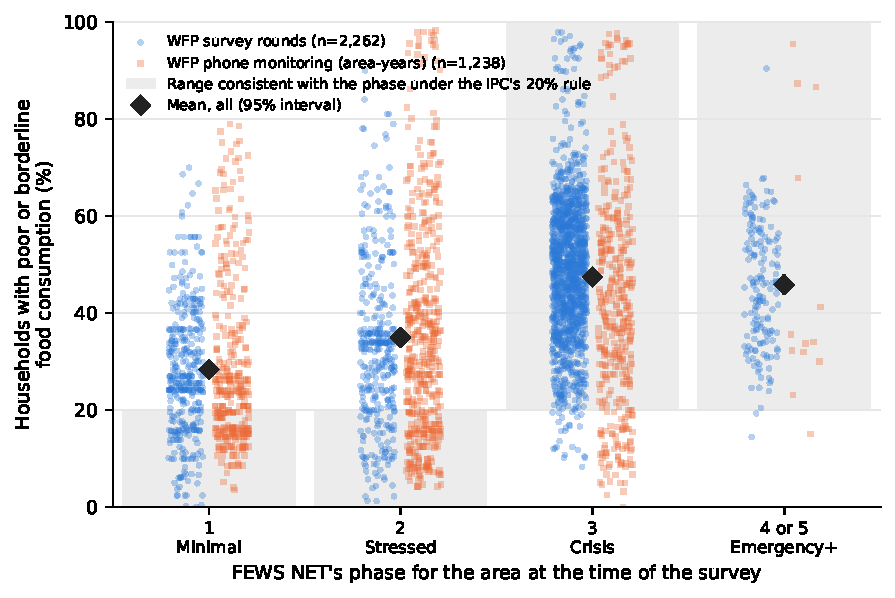
\includegraphics[width=0.9\textwidth]{figures/fig9g_phase_fcs.pdf}
\caption{Household food consumption by FEWS NET phase. Each point is one area in one WFP survey round (blue), one area-year of WFP's monthly phone monitoring (orange), or one area in one round of FAO's DIEM household surveys (green): the share of households with poor or borderline food consumption, against the phase FEWS NET's map gave the area at the time (mean over the FEWS NET units in the area, rounded; points jittered). Data: WFP, compiled in the Joint Research Centre's harmonized food insecurity dataset and WFP's monitoring files, by region, 2011--2024; FAO DIEM, \dmYearZero{}--\dmYearOne{}. Grey boxes: the range consistent with each phase under the IPC's rule that an area is in a phase when at least 20 percent of its households are in that phase or worse, with borderline consumption counted as Crisis and poor consumption as Emergency or worse; below 20 percent for Phases 1 and 2, at least 20 percent for Crisis or worse (this indicator cannot separate Crisis from Emergency). Diamonds: means with 95 percent intervals.}\label{fig:phfcs}
\end{figure}

\begin{figure}[t]
\centering
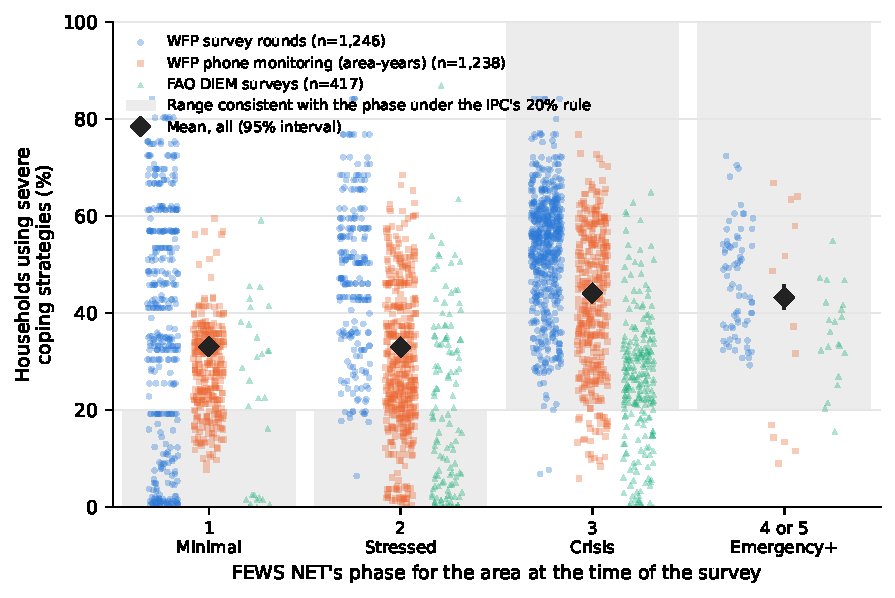
\includegraphics[width=0.9\textwidth]{figures/fig9h_phase_rcsi.pdf}
\caption{Household coping by FEWS NET phase. As Figure~\ref{fig:phfcs}, for the share of households using severe consumption coping strategies (reduced coping strategies index of 19 or more, which the IPC's reference table places at Crisis or worse). Grey boxes: the range consistent with each phase under the IPC's 20 percent rule.}\label{fig:phrcsi}
\end{figure}

Where the phases and the indicators disagree, the phases are milder. Under the IPC's 20 percent rule, \fsFcsLowOver{} percent of areas mapped in Phases 1 or 2 had too many households with poor or borderline consumption for their phase, and \fsRcsiLowOver{} percent had too many coping severely; only \fsFcsHighUnder{} and \fsRcsiHighUnder{} percent of areas mapped in Crisis or worse had too few. The indicators are consistent with the classification in Crisis areas and much worse than it in areas called Minimal or Stressed. This fits \citet{Lentz2025undercount}, who find that official estimates undercount acute hunger, and \citet{lentz2024ipcaccuracy}, who find the IPC's analyses only partly consistent with their own evidence. It does not prove the phases wrong: survey indicators are noisy, and analysts weigh other evidence. But it means that, if anything, phase counts understate household food insecurity.

FAO's DIEM surveys, which began after most of the WFP data end, show the same pattern on their own. Across \dmRounds{} area-rounds in \dmCountries{} countries, the share of households with poor or borderline food consumption averages \dmFcsOne{} percent in areas FEWS NET mapped as Minimal and \dmFcsFour{} percent in areas in Emergency or worse; it correlates \dmFcsCorr{} with FEWS NET's phase across areas and \dmFcsCorrArea{} within an area over time, and \dmFcsLowOver{} percent of areas mapped Minimal or Stressed have 20 percent or more of households at Crisis level. The two indicators the WFP data lack tell the same story. Moderate or severe hunger averages \dmHhsOne{} percent in Minimal areas and \dmHhsFour{} percent in Emergency, with correlations of \dmHhsCorr{} across areas and \dmHhsCorrArea{} within them; crisis or emergency livelihood coping averages \dmLcsOne{} and \dmLcsFour{} percent, with correlations of \dmLcsCorr{} and \dmLcsCorrArea{}. Against the official IPC or Cadre Harmonis\'e phase rather than FEWS NET's, the correlations across areas are similar (\dmFcsIpcCorr{} for food consumption, \dmHhsIpcCorr{} for hunger, \dmLcsIpcCorr{} for livelihood coping) and within areas over time close to zero (\dmFcsIpcCorrArea{}, \dmHhsIpcCorrArea{}, \dmLcsIpcCorrArea{}). FAO notes that these surveys feed IPC analyses, so they are not independent of the classifiers' evidence; that makes the weak link more striking, not less.

The analysts' own inputs tell the same story. Even the indicators Cadre Harmonis\'e analysts recorded for an area correlate only loosely with the phase those analysts assigned: \chFcsCorr{} for poor or borderline food consumption, \chHhsCorr{} for moderate or severe household hunger, \chLcsCorr{} for crisis livelihood coping and \chRcsiCorr{} for severe consumption coping. A phase is a consensus that weighs several kinds of evidence and adjusts for context. Its link to any single measured outcome is correspondingly loose. That is defensible for a summary of food insecurity. It is a problem when the phase is used as a proxy for outcomes it does not directly weigh.

\section{Phases and child malnutrition}\label{sec:gam}

Somalia's scheduled surveys give the cleanest test. Mean acute malnutrition among children under five was \fsGamTwo{} percent in zones FEWS NET forecast to be Stressed or better, \fsGamThree{} percent in zones forecast to be in Crisis, and \fsGamFour{} percent in zones forecast to be in Emergency or worse (Figure~\ref{fig:phgam}, blue points). The IPC bands for those phases are 5--10, 10--15 and 15--30 percent. The correlation between the forecast and the measured rate is \fsCorrFc{}. The correlation with FEWS NET's map published just after the survey, which could draw on its results, is \fsCorrAfter{}.

\begin{figure}[t]
\centering
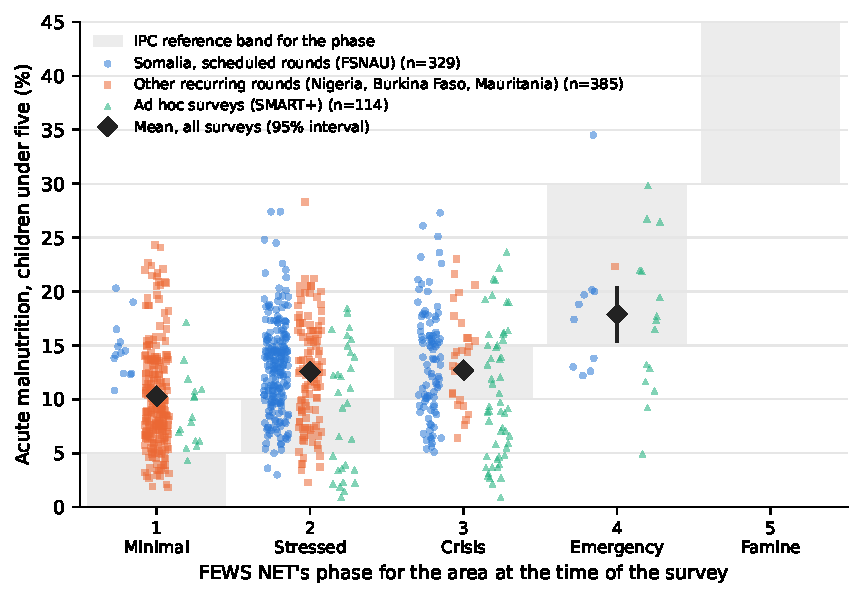
\includegraphics[width=0.9\textwidth]{figures/fig9a_phase_gam.pdf}
\caption{Measured acute malnutrition by FEWS NET phase. Each point is one survey: global acute malnutrition (weight-for-height) among children under five, against the phase FEWS NET's map gave the area at the time of the survey (rounded mean over the FEWS NET units in the survey area; points jittered). Grey boxes: the IPC reference band for each phase. Blue: Somalia's scheduled FSNAU rounds, rural zones, 2011--2024. Orange: other recurring national or sub-national rounds (Nigeria's UNICEF rounds, 2023--26; Burkina Faso and Mauritania national rounds, 2003--18). Green: ad hoc surveys in the SMART+ dashboard, 2022--26. Diamonds: mean of all surveys in the phase, with 95 percent intervals.}\label{fig:phgam}
\end{figure}

Comparing zones with each other could hide a gradient over time, since some zones always have high malnutrition. So we also compare each zone with itself. When FEWS NET forecast a zone to be one phase worse than usual, its acute malnutrition was \wzGamZone{} points higher (standard error \wzGamZoneSe{}), or \wzGamZoneSeason{} points with season effects removed (Appendix Figure~\ref{fig:within}). The bands imply 5 points for a step from Stressed to Crisis and 10 for a step from Crisis to Emergency. The estimate may be biased down, because a survey zone's phase averages several FEWS NET units and the worst-hit zones are under-surveyed; but it is consistent with \citet{reusken2025}, who find a link between the official Phase 3+ share and later malnutrition in Somali districts that is real but far weaker than the bands.

Other countries show a steeper gradient, still well below the bands. In SMART+ surveys, mean acute malnutrition was \spGamOne{}, \spGamTwo{}, \spGamThree{} and \spGamFour{} percent across Phases 1, 2, 3 and 4 or worse, and one phase goes with \spSlope{} points (standard error \spSlopeSe{}) with country-by-year effects; the jump at Phase 4 comes mostly from a dozen ad hoc surveys in Ethiopia. Nigeria's recurring rounds give \ngSlope{} points per Cadre Harmonis\'e phase, and the Burkina Faso and Mauritania rounds \fdwSlope{} per FEWS NET phase. The IPC's two scales tell the same story from the inside: where an area has both a food insecurity phase and an acute malnutrition phase for the same period, they agree only \amnAnyDiag{} percent of the time, and areas the food insecurity scale calls Crisis are spread almost evenly across all four malnutrition phases (Appendix Figure~\ref{fig:amn}).

\section{Phases and death}\label{sec:death}

For mortality the link is weaker still. In the SMART+ surveys that measured it, crude death rates were \spCdrOne{}, \spCdrTwo{}, \spCdrThree{} and \spCdrFour{} deaths per 10,000 people per day in areas FEWS NET mapped in Phases 1, 2, 3 and 4 or worse: flat, with a slope of \spCdrSlope{} (standard error \spCdrSlopeSe{}) (Figure~\ref{fig:phcdr}). Against the official IPC or Cadre Harmonis\'e phase they rise by \spCdrSlopeIpc{} per phase (\spCdrSlopeIpcSe{}). The IPC bands step by 0.5 to 1 per phase. Within Somali zones, a phase worse than usual goes with \wzCdrZone{} more deaths per 10,000 per day (\wzCdrZoneSe{}), where the bands imply 0.45--0.75.

\begin{figure}[t]
\centering
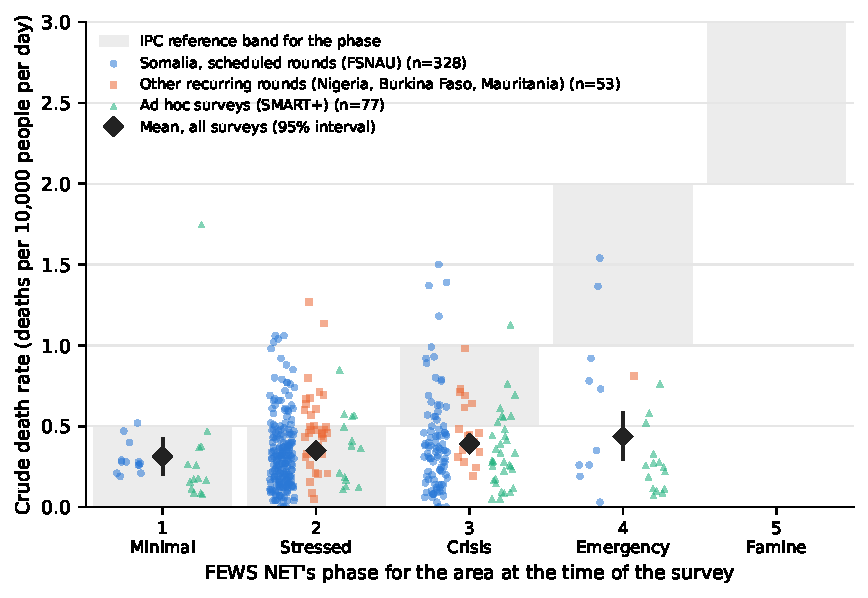
\includegraphics[width=0.9\textwidth]{figures/fig9b_phase_cdr.pdf}
\caption{Measured crude death rates by FEWS NET phase. As Figure~\ref{fig:phgam}, for crude death rates (deaths per 10,000 people per day), in surveys that measured mortality. Grey boxes: the IPC reference band for each phase.}\label{fig:phcdr}
\end{figure}

The crises whose death tolls have been estimated point the same way (Figure~\ref{fig:excess}). Dividing excess deaths by the number of people in Crisis or worse gives an excess death rate per person in Phase 3 or worse of roughly 0.15--0.2 per 10,000 per day in Somalia's 2017--18 and 2022 droughts, about 0.9 in northeast Nigeria in 2016--19, and 1.1--1.9 in the 2010--12 Somalia famine, which met a late response \citep{warsame2023,lshtm2023somalia,checchi2023nigeria,checchi2013}. The two droughts in which aid arrived at scale sit well below the IPC's Crisis band; the two cases above it are a famine with a late response and a conflict. Measured crude death rates in areas reviewed for famine since 2017 have mostly been between 0.3 and 1.9, below the famine threshold of 2 \citep{ipcfrc2022somaliadec,ipcfrc2024sudandec}.

\begin{figure}[t]
\centering
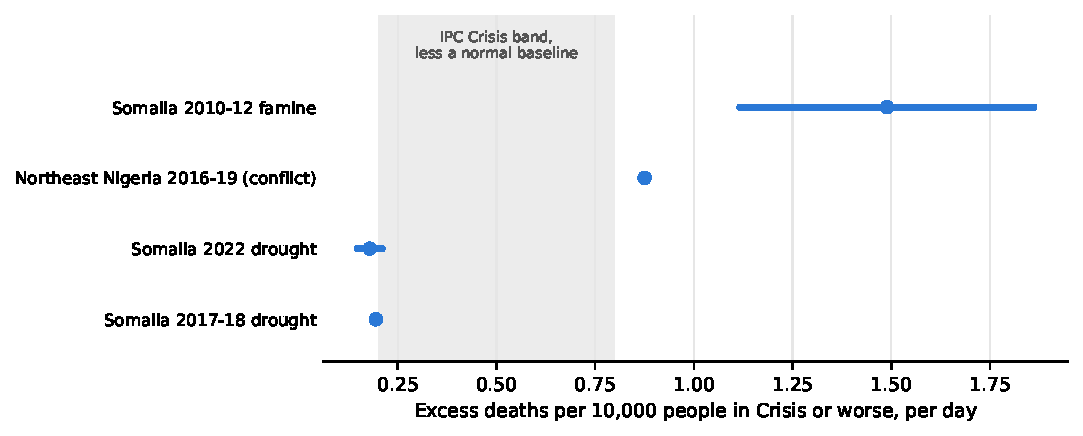
\includegraphics[width=0.85\textwidth]{figures/fig9f_excess_deaths.pdf}
\caption{Excess deaths in documented crises, per person in Crisis or worse. Estimated excess deaths divided by the number of people classified in IPC or Cadre Harmonis\'e Phase 3 or worse and the length of the crisis; ranges reflect ranges in the death toll and in the Phase 3+ population. Grey band: the IPC Crisis band for crude death rates (0.5--1 per 10,000 per day) less a normal baseline of 0.2--0.3. Sources: \citet{warsame2023,lshtm2023somalia,checchi2023nigeria,checchi2013}.}\label{fig:excess}
\end{figure}

Death rates in crises vary enormously, and the phase captures little of that variation. Arithmetic with the bands would have predicted roughly two to five times the excess deaths estimated for Somalia in 2022. A death toll inferred from a phase count is not a measurement.

\section{Why the link is weak}\label{sec:why}

The simplest explanation is that phases measure food insecurity well enough, and that food insecurity is only one cause of malnutrition and death in crises.

\paragraph{What people die of.} Since Alex de Waal's study of the 1984--85 Darfur famine, the consensus in humanitarian public health has been that most excess deaths in famines are not deaths from starvation. In Darfur the crude death rate roughly trebled, mostly through a seasonal spike in child deaths from diarrhoea, measles and malaria, and access to water predicted who died better than wealth did \citep{dewaal1989famine,dewaal1989popstud}. Studies of refugee and displaced populations in the 1980s and 1990s found the same four killers --- measles, diarrhoea, respiratory infection and malaria --- made deadlier by malnutrition \citep{toole1990,toole1997}. Economic historians find the same profile in Ireland, India and Russia before antibiotics \citep{mokyr2002}. In Gode, Ethiopia, in 2000, measles alone or combined with malnutrition caused about a fifth of under-five deaths, and a measles campaign was mounted only after the bulk of food aid had arrived \citep{salama2001}. In Darfur in 2003--08, more than 80 percent of an estimated 300,000 excess deaths were not violent, mostly diarrhoea among the displaced \citep{degomme2010}. Across 1,759 death rate estimates from crises between 1998 and 2012, non-violent excess deaths outnumber violent ones even in exceptionally brutal conflicts \citep{heudtlass2016}.

\paragraph{What predicts malnutrition and death.} The best statistical models of crisis mortality, fitted for Somalia, South Sudan and northeast Nigeria, lean on conflict, measles, malaria, displacement and admissions for severe malnutrition; none uses the IPC phase as a predictor \citep{Checchi2022SAE,checchi2023nigeria}. Models of acute malnutrition in Somalia and South Sudan found livelihood, measles, vegetation, terms of trade and water prices most useful, and still performed poorly \citep{checchi2022malnut}. Wasting in Somalia peaks around May--June and November and falls during the lean season, so it does not follow the food insecurity calendar \citep{luc2024fex}; wasting peaks across Africa track heat and disease seasons more than the hunger gap \citep{venkat2023seasonality}. In parts of Chad and South Sudan, acute malnutrition has stayed above the 15 percent emergency threshold for decades, including when the IPC classified the area as Minimal \citep{youngmarshak2017}. A meta-analysis of household studies finds that food insecurity predicts stunting and underweight but not wasting \citep{moradi2019}.

\paragraph{Why the bands are too steep.} The bands came from camps, where populations were crowded, newly displaced and often hit by epidemics, and where death rates rose steeply with wasting \citep{youngjaspars2009}. The IPC applies them to whole rural livelihood zones whose baselines and disease environments differ. In south-central Somalia in 2010--12, death rates in areas classified Minimal or Stressed were already 0.5--0.8 per 10,000 per day, inside the Crisis band \citep{checchi2013}. The same absolute bands make the opposite error where baselines are low: in Gaza, a death rate meeting the Famine threshold would have required a more than twentyfold rise, against six- to sevenfold in rural Somalia \citep{deZwarte2026Lancet}. Both problems come from fixing absolute death rates to phases defined by food.

\paragraph{What it takes to be classified in Crisis.} The classification itself shows where malnutrition and death enter. For 2021--2023, the Cadre Harmonis\'e's public file records the evidence behind each of its \cxAreaN{} current area classifications in \cxCountries{} countries: household shares on each indicator, the phase its analysts gave each indicator, the phase they gave each dimension (food consumption, livelihoods, nutrition and mortality), and the area's phase. The chain has three steps. First, for dietary diversity, household hunger, reduced coping and livelihood coping, the analysts' phase for the indicator follows the IPC's 20 percent rule almost mechanically (\cxRuleHdds{}, \cxRuleHhs{}, \cxRuleRcsi{} and \cxRuleLcs{} percent of cases). For food consumption they use a more lenient threshold: areas they put at Crisis on this indicator have a median of \cxFcgMedThree{} percent of households with poor or borderline consumption. Second, when the four food consumption indicators disagree, the dimension's phase matches the least severe of them in \cxDimMin{} percent of cases and the most severe in only \cxDimMax{} percent. Third, the area's phase equals the food consumption phase in \cxAreaFood{} percent of cases and is never worse than the worst dimension. Table~\ref{tab:chcells} shows what it takes. No area with Minimal food consumption is classified in Crisis, whatever its livelihoods; with Stressed food consumption it takes emergency-level livelihood coping, and then only half the time. The food consumption and livelihood phases together explain \cxRtwoCells{} percent of the variation in whether an area is placed in Crisis or worse. Holding them fixed, a nutrition phase of Crisis or worse raises the chance by \cxNut{} percentage points (standard error \cxNutSe{}) and a mortality phase of Crisis or worse by \cxMort{} (\cxMortSe{}); together they raise the explained share only to \cxRtwoAll{} percent. Of the \cxNutFoodOneN{} areas where analysts found serious or critical acute malnutrition but Minimal food consumption, \cxNutFoodOneP{} percent were classified in Crisis. In the system's own records, malnutrition and mortality are evidence that rarely moves the phase; the phase is a measure of food consumption and coping.

\begin{table}[t]
\centering
\caption{Share of Cadre Harmonis\'e areas classified in Crisis or worse (Phase 3+), by the phases its analysts gave the food consumption and livelihood dimensions, 2021--2023. Number of area classifications in parentheses.}\label{tab:chcells}
\small
\begin{tabular}{lcccc}
\toprule
 & \multicolumn{4}{c}{Livelihoods phase} \\
\cmidrule(lr){2-5}
Food consumption phase & 1 Minimal & 2 Stressed & 3 Crisis & 4 Emergency \\
\midrule
1 Minimal & \cxCellAA\% (\cxCellAAN) & \cxCellAB\% (\cxCellABN) & \cxCellAC\% (\cxCellACN) & \cxCellAD\% (\cxCellADN) \\
2 Stressed & \cxCellBA\% (\cxCellBAN) & \cxCellBB\% (\cxCellBBN) & \cxCellBC\% (\cxCellBCN) & \cxCellBD\% (\cxCellBDN) \\
3 Crisis & \cxCellCA\% (\cxCellCAN) & \cxCellCB\% (\cxCellCBN) & \cxCellCC\% (\cxCellCCN) & \cxCellCD\% (\cxCellCDN) \\
4 Emergency & -- & -- & \cxCellDC\% (\cxCellDCN) & \cxCellDD\% (\cxCellDDN) \\
\bottomrule
\end{tabular}
\begin{minipage}{0.92\textwidth}\footnotesize\smallskip
Source: Cadre Harmonis\'e consolidated dataset (current analyses; Central African Republic excluded). \cxNutN{} of the classifications also record a nutrition phase and \cxMortN{} a mortality phase.
\end{minipage}
\end{table}

\paragraph{Where food does matter.} None of this says that food does not matter. In sieges and in populations with good water and health services, starvation itself can dominate, as in the European famines of the 1940s \citep{mokyr2002}, and plausibly in Gaza. At the extreme, as in Somalia in 2011, food deprivation and disease compound each other, and the presence of food aid lowered death rates \citep{checchi2013}. Preventive food supplements and cash can reduce wasting at the margin \citep{isanaka2009rutf,langendorf2014preventing}. Our claim is narrower: across the large populations in Crisis and Emergency where most crisis deaths occur, the amount of food insecurity explains little of the variation in who becomes malnourished or dies.

\paragraph{Where the money goes.} Humanitarian funding follows the food-insecurity frame. Across \ftsYearZero{}--\ftsYearOne{}, the food security cluster received \ftsFood{} percent of all humanitarian funding reported to OCHA's Financial Tracking Service, health \ftsHealth{} percent, nutrition \ftsNutrition{} percent, and water, sanitation and hygiene \ftsWash{} percent; about \ftsUntagged{} percent was not assigned to a sector. Some of the food money saves lives, and some of it buys nutrition and health benefits. But if most deaths come from disease, a system that sizes and prioritizes crises by counts of food-insecure people is aiming at a small part of the problem.

\section{Where the money goes}\label{sec:money}

If phases are a weak guide to malnutrition and death, the question is whether aid follows them anyway. We look at three levels, with three information sets: the phases; triggers of crisis (rainfall, conflict and prices, described in Section~\ref{sec:surveys}); and the outcomes measured in surveys. Aid is measured in total, across sectors, since a reallocation toward malnutrition and death need not respect the boundaries between food, nutrition, health and water. We report three things. The first is how well each information set predicts where aid goes, scored out of sample as in equation~(\ref{eq:predict}), with the share of aid each place receives in a season as the outcome. The second is a horse race. For location $d$ in season $s$, with aid $A_{ds}$ per person (scaled per person, per 100,000 people or per 1,000 people for dollars, organizations and people reached),
\begin{equation}\label{eq:aid}
\log(1 + A_{ds}) = \lambda_s + \beta_P P_{ds} + \beta_G G_{ds} + \beta_C C_{ds} + \beta_U U_{ds} + \rho \log N_{ds} + [\mu_d] + \varepsilon_{ds},
\end{equation}
where $P$ is the standardized Phase 3+ share, $G$, $C$ and $U$ the standardized acute malnutrition, crude death and under-five death rates measured in the survey that season, and $N$ population, with standard errors clustered by location. Aid is measured in the six months after the survey, so all of these are known first. Without location effects $\mu_d$, the season effects $\lambda_s$ make this a comparison \emph{between} locations in the same season: do places with more people in Phase 3 or more deaths get more aid? With them, it compares each location with itself over time: when a place's phase or death rate rises, does its aid rise? The third is how much aid would have to move for its distribution to match each measure of need $n$: the dissimilarity index $\tfrac12 \sum_d |A_{ds}/\sum_d A_{ds} - n_{ds}/\sum_d n_{ds}|$, averaged over seasons, where $n$ is people in Phase 3 or worse, expected deaths (the crude death rate times population), expected under-five deaths, or acutely malnourished children.

\paragraph{Across countries.} For \xcCountries{} countries in the Global Report on Food Crises, \xcYearZero{}--\xcYearOne{}, we compare humanitarian funding reported to OCHA with the number of people in Phase 3 or worse, under-five deaths and battle deaths:
\begin{equation*}
\log F_{ct} = \lambda_t + \beta_P \log P_{ct} + \beta_U \log U_{ct} + \beta_B \log(1 + B_{ct}) + \rho \log N_{ct} + \varepsilon_{ct},
\end{equation*}
for country $c$ in year $t$, with funding $F$, Phase 3+ population $P$, under-five deaths $U$, battle deaths $B$ and population $N$. Within a year and holding population fixed, funding has an elasticity of \xcElastPthree{} (standard error \xcElastPthreeSe{}) with respect to the Phase 3+ population and \xcElastBattle{} (\xcElastBattleSe{}) with respect to battle deaths; with respect to under-five deaths it is \xcElastUfive{} (\xcElastUfiveSe{}). For funding to be distributed across countries like people in Phase 3 or worse, \xcDisPthree{} percent of it would have to move; like under-five deaths, \xcDisUfive{} percent. The death figures here are modelled national estimates that include deaths in normal times, so this comparison says only that funding follows hunger counts and conflict, not where children die.

\paragraph{Within Somalia.} Districts are the unit, in each of \arSomUsdPeriods{} survey seasons from 2015. Aid is measured in the six months after each survey, so every predictor is known first: OCHA's pooled-fund budgets by district, the number of organizations present (OCHA's who-does-what-where reports) and the number of people reached. Pooled-fund budgets, a few percent of all funding, are too lumpy to be predicted by anything (Figure~\ref{fig:aidr2}). Organizations' presence follows population (out-of-sample $R^2$ of \arSomPrtBase{}); the phases, the triggers and the surveys each add little to that. Where the phases and the outcomes disagree, aid follows the phases, both between districts and within them. Between districts in the same season (equation~\ref{eq:aid} without location effects), a district whose Phase 3+ share is one standard deviation higher has about \hrSomPrtPthree{} log points more organizations per person (standard error \hrSomPrtPthreeSe{}) and reaches \hrSomRchPthree{} log points more people (\hrSomRchPthreeSe{}), holding measured outcomes fixed; a district whose under-five death rate is one standard deviation higher, holding the Phase 3+ share fixed, has \hrSomPrtUfive{} log points more organizations (\hrSomPrtUfiveSe{}) and reaches \hrSomRchUfive{} log points more people (\hrSomRchUfiveSe{}), that is, fewer. Within districts over time (with location effects), when a district's Phase 3+ share rises by one standard deviation it gains \hrWSomPrtPthree{} log points of organizations (\hrWSomPrtPthreeSe{}) and \hrWSomRchPthree{} of people reached (\hrWSomRchPthreeSe{}); when its under-five death rate rises by one standard deviation, its organizations change by \hrWSomPrtUfive{} log points (\hrWSomPrtUfiveSe{}): they fall. Acute malnutrition is the one outcome aid responds to within districts: pooled-fund dollars rise by \hrWSomUsdGam{} log points (\hrWSomUsdGamSe{}) and organizations by \hrWSomPrtGam{} (\hrWSomPrtGamSe{}) per standard deviation, as one would expect of nutrition programmes that size their caseloads from surveys.

For aid's distribution to match people in Phase 3 or worse, \disSomPrtPthree{} percent of organizations' presence and \disSomRchPthree{} percent of people reached would have to move between districts in a season. To match expected deaths it would be \disSomPrtDeaths{} and \disSomRchDeaths{} percent, to match expected under-five deaths \disSomPrtUfive{} and \disSomRchUfive{} percent, and to match acutely malnourished children \disSomPrtMaln{} and \disSomRchMaln{} percent. Aid is distributed more like people in Phase 3 or worse --- and like population, \disSomPrtPop{} and \disSomRchPop{} percent --- than like deaths.

\paragraph{Within northeast and northwest Nigeria.} Using the national nutrition surveillance rounds since 2023 and aid by local government area, Nigeria does not show the same pattern. Pooled-fund budgets rise with both the Cadre Harmonis\'e Phase 3+ share and measured crude death rates, and measured outcomes predict where organizations are present (out-of-sample $R^2$ of \arNgaPrtSurv{}) better than the phases do (\arNgaPrtPhase{}). Aid's distribution is about as close to expected deaths as to people in Phase 3 or worse (\disNgaPrtDeaths{} against \disNgaPrtPthree{} percent of organizations' presence would have to move). Within local government areas over time, neither the phases nor the outcomes predict changes in aid. Nigeria's surveillance rounds are recent, and organizations' presence is recorded only in the northeast, so this is a small sample; it shows that following measured outcomes is possible, not that it is common.

\begin{figure}[t]
\centering
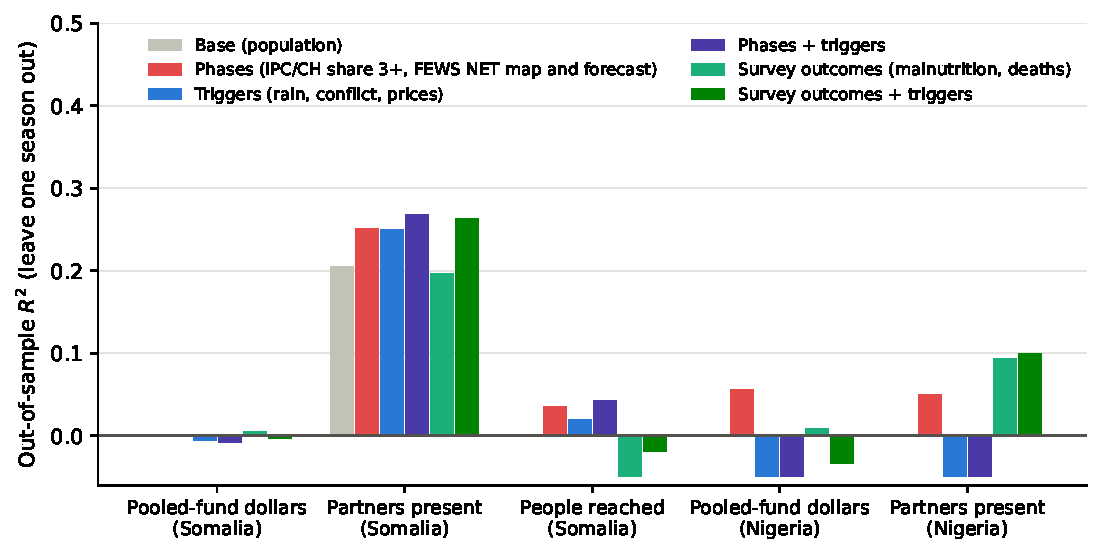
\includegraphics[width=0.9\textwidth]{figures/fig14_aid_r2.pdf}
\caption{What predicts where aid goes? Out-of-sample $R^2$ (leaving one survey season out) of the share of aid each district (Somalia) or local government area (Nigeria) receives in the six months after a survey, relative to the season's average, for each information set at the time of the survey. All models include log population. Aid is measured across all sectors: OCHA pooled-fund budgets, organizations present (OCHA 3W) and people reached (Somalia only). Information sets as in Figure~\ref{fig:triggers}, with survey outcomes measured in the same season. Somalia: \arSomPrtUnits{} districts, 2015--2026; Nigeria: \arNgaUsdUnits{} local government areas, 2023--2026.}\label{fig:aidr2}
\end{figure}



\section{What surveys add}\label{sec:surveys}

If phases say little about malnutrition and death, what does? The simplest predictor of a zone's acute malnutrition is its last survey. In Somalia, a zone's result six months earlier correlates \fsCorrLag{} with this round's (Appendix Figure~\ref{fig:persist}). Out of sample, leaving out one season at a time, the previous survey explains \fsRtwoLag{} of the variance in acute malnutrition and FEWS NET's forecast explains none ($R^2$ of \fsRtwoFc{}); adding the forecast to the previous survey does not help (\fsRtwoBoth{}). Given one zone that reaches the critical level of 15 percent and one that does not, the previous survey ranks them correctly \fsAucLag{} of the time; the forecast does no better than a coin toss (\fsAucFc{}). The same holds for under-five death rates: an out-of-sample $R^2$ of \fsMortLag{} for the previous survey and \fsMortFc{} for the forecast. Models that try to predict malnutrition without recent surveys, from rainfall, prices, conflict and disease, have performed poorly \citep{checchi2022malnut}.

FEWS NET barely uses this information. A Somali zone whose last survey showed 10 more points of acute malnutrition was forecast \fsFcOnLag{} of a phase worse (standard error \fsFcOnLagSe{}). That is not a failure of FEWS NET's analysts: their scale is about food insecurity, and survey results about malnutrition do not translate into it. Where surveys do move FEWS NET's maps, they move them in one direction only. In Somalia, Ethiopia and Sudan, \svTotal{} survey results are quoted in FEWS NET's reports; when one was carried out between a forecast and the next map, that map was \nsUp{} percentage points (standard error \nsUpSe{}) more likely to be worse than forecast, from a base of \nsUpBase{} percent, and no more likely to be better. Surveys showing acute malnutrition below 15 percent moved the maps up about as much as alarming ones (\nsOkUp{} against \nsCritUp{} points). Agencies send survey teams where they suspect trouble, and the decision to survey is itself the signal. That is useful, but it is not the same as measuring.

\paragraph{Could cheaper signals do the job?} Surveys are costly and do not go everywhere (Section~\ref{sec:gaps}). Drought, conflict and prices are observed everywhere, from satellites, conflict-event databases and markets. Do they predict malnutrition and death in ways the phases miss? We test this in Somalia, on \trN{} survey domains and seasons from \trYearZero{} to \trYearOne{} --- rural zones, towns and displaced settlements --- where we observe the official IPC share of the population in Phase 3 or worse, FEWS NET's map and forecast, and the triggers: rainfall anomalies over 6 and 12 months, conflict fatalities over 6 months, and cereal and goat prices, all measured up to the survey month.

For survey domain $a$ in season $s$, with outcome $y_{as}$ and information set $x^k_{as}$ (the phases, the triggers or the previous survey), we estimate
\begin{equation}\label{eq:predict}
y_{as} = \alpha + \gamma' b_{as} + \theta_k' x^k_{as} + \varepsilon_{as},
\end{equation}
where $b_{as}$ indicates the population type (rural zone, town, displaced settlement) and season type, on all seasons but $s$, and predict $\hat y^{(-s)}_{as}$ for the season left out. The out-of-sample $R^2$ is $1 - \sum (y_{as} - \hat y^{(-s)}_{as})^2 / \sum (y_{as} - \bar y)^2$; it is negative when an information set predicts worse than the overall mean. Every information set is scored on the same observations.

The triggers beat the phases (Figure~\ref{fig:triggers}). Predicting each season's surveys from the others, the triggers explain \trGamTrig{} of the variance in acute malnutrition and \trUfiveTrig{} in under-five death rates; the phases explain \trGamPhase{} and \trUfivePhase{}, no better than knowing the population type and season. Conflict alone does most of the work (\trSingleConfGam{} and \trSingleConfUfive{}). The previous survey is still the best single guide to malnutrition (\trGamLast{}), but for death rates the triggers add to it (\trUfiveLast{} with the previous survey alone, \trUfiveLastTrig{} with the triggers). For a place never surveyed --- predicting a domain from all the others, beyond the season's national average --- the phases add nothing for any outcome, the triggers improve the prediction of acute malnutrition modestly ($R^2$ of \ldGamTrig{}; \ldSamTrig{} for severe malnutrition), and nothing we have predicts death rates (\ldCdrTrig{} and \ldUfiveTrig{}).

Within a domain over time, drought is the trigger that matters, and the phases do not respond to it. We estimate
\begin{equation}\label{eq:within}
y_{as} = \beta' z_{as} + \delta\, P_{as} + \mu_a + \kappa\, \textit{Deyr}_s + \tau t_s + \varepsilon_{as},
\end{equation}
where $z_{as}$ are the standardized triggers, $P_{as}$ the standardized IPC Phase 3+ share, $\mu_a$ domain effects, \textit{Deyr}$_s$ the season type and $t_s$ a linear trend, with standard errors clustered by domain. We use a trend rather than season effects because droughts hit much of the country at once, and season effects would absorb them. With these controls, a 12-month rainfall deficit of one standard deviation goes with \twGamDry{} more points of acute malnutrition (standard error \twGamDrySe{}), \twSamDry{} more points of severe malnutrition (\twSamDrySe{}), \twCdrDry{} more deaths per 10,000 per day (\twCdrDrySe{}), and \twMorbDry{} more points in the share of children ill in the previous two weeks (\twMorbDrySe{}), holding the IPC share fixed. The IPC share itself responds to conflict and cereal prices --- one standard deviation more conflict raises it by \tpFat{} points (\tpFatSe{}) --- but not to the 12-month rainfall deficit (\tpDry{} points, standard error \tpRainyrSe{}). The phases are not noise: within a domain, a higher IPC share still goes with more severe malnutrition and higher death rates (\twCdrPthree{} deaths per 10,000 per day per standard deviation, \twCdrPthreeSe{}). But the signals the classification weighs are the food signals, prices and conflict, while drought reaches children's bodies partly through illness, which the classification does not count.

Two lessons follow. Cheap triggers carry information about malnutrition that the phases do not, so a system aiming at malnutrition could use them to decide where to look. But they do not substitute for measurement: in places without surveys, no signal we have predicts how many people are dying. We repeated the comparison for Nigeria's nutrition surveillance rounds, \ngN{} survey domains and rounds since 2023; the sample is too small and too recent for any information set, phases included, to predict outcomes out of sample.

\begin{figure}[t]
\centering
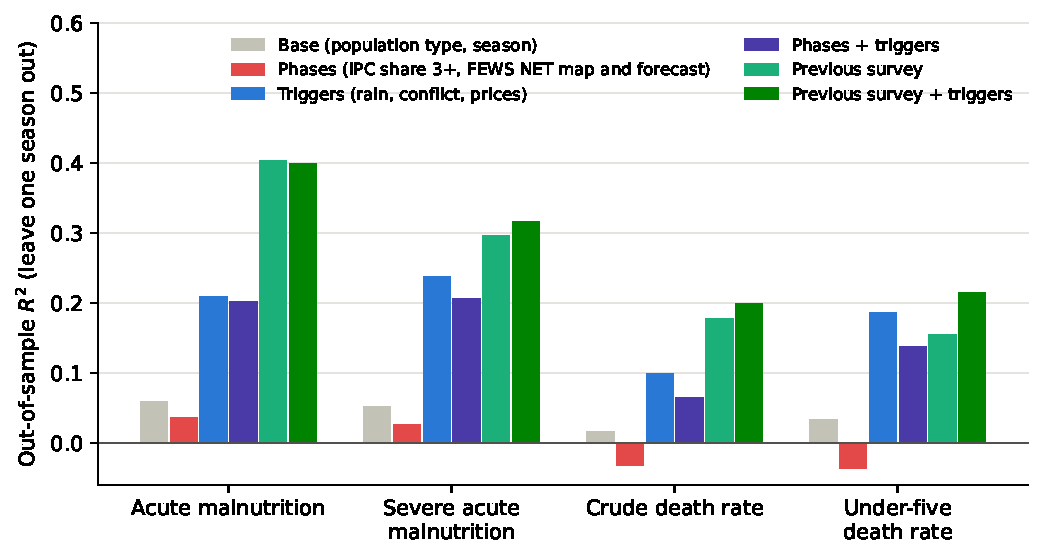
\includegraphics[width=0.85\textwidth]{figures/fig13_triggers_r2.pdf}
\caption{What predicts malnutrition and death in Somalia's surveys? Out-of-sample $R^2$ from predicting each season's survey results with a model fitted on the other seasons, by information set, for the same \trN{} survey domains and seasons, \trYearZero{}--\trYearOne{} (rural zones, towns and displaced settlements). All models include population type (rural, town, displaced) and season type. Phases: official IPC share of the population in Phase 3 or worse, and FEWS NET's current map and forecast. Triggers: CHIRPS rainfall anomalies over 6 and 12 months, log ACLED conflict fatalities over 6 months, and log cereal and goat prices over 3 months, all up to the survey month. Previous survey: the domain's own outcome, morbidity and measles vaccination coverage in its previous survey. Negative values are shown at the axis.}\label{fig:triggers}
\end{figure}

\paragraph{Is aid hiding the phases' value?} These comparisons share an identification problem. Droughts and conflicts feed both the surveys and the phases. Aid follows the phases more than the surveys, at least in Somalia. If aid works, it lowers malnutrition and death where the phases sent it, so the phases will look like worse predictors of outcomes than they are of the outcomes that would have occurred without aid; some of their apparent false alarms may be successes. Separating these would need variation in aid unrelated to need, which we do not have. Instead we ask how effective aid would have to be to overturn the result.

We rebuild each survey's outcome as it would have been without aid, adding back the deaths and malnutrition that aid would have averted, and rerun the horse race of equation~(\ref{eq:predict}) on these counterfactual outcomes $y^*$. Let $A_{as}$ be humanitarian aid per person reaching domain $a$ in the six months before season $s$'s survey. If aid averts a death for every \$$c$ spent and $m$ cases of acute malnutrition per death, and a share $\phi$ of averted deaths are children under five, who make up a share $\pi$ of the population, the counterfactual crude death rate, under-five death rate (both per 10,000 per day) and acute malnutrition prevalence (percent) are
\begin{align}
\textit{CDR}^*_{as} &= \textit{CDR}_{as} + \frac{A_{as}}{c} \cdot \frac{10^4}{182.5}, \nonumber\\
\textit{U5DR}^*_{as} &= \textit{U5DR}_{as} + \frac{\phi}{\pi}\cdot\frac{A_{as}}{c} \cdot \frac{10^4}{182.5}, \label{eq:bounds}\\
\textit{GAM}^*_{as} &= \textit{GAM}_{as} + \frac{100\, m}{\pi} \cdot \frac{A_{as}}{c}, \nonumber
\end{align}
with $\phi = 0.5$ (as in Somalia in 2022), $\pi = 0.19$ and $m = 10$. The previous survey enters the prediction as $y^*$ for the previous season too. We take the case least favorable to our argument:
\begin{equation*}
A_{as} = \bar A_{t(s)} \cdot \frac{P_{as}}{\overline{P}_s},
\end{equation*}
that is, all humanitarian funding reported for Somalia in the year, $\bar A$, about \$\bdNatPc{} per person per six months, allocated across domains in exact proportion to the IPC Phase 3+ share $P_{as}$ relative to the season's average. Aid then lines up perfectly with the phases, and the phases get full credit for every death it averts. We vary $c$ from infinity (aid does nothing) down to \$250 (Figure~\ref{fig:bounds}). If aid averts no deaths, the phases lose, as before. They catch up with the previous survey in predicting counterfactual death rates only if all humanitarian aid averts a death for about \bdBreakCdrLast{} (crude death rate) to \bdBreakUfiveLast{} (under-five death rate) or less. That is as cheap as the best-evidenced life-saving intervention in crises, community treatment of severe acute malnutrition, at roughly \$4,000--7,000 per death averted \citep{givewell2024cmam,givewell2024taimaka}; most humanitarian spending, from food rations to logistics, is surely far less cost-effective per death. For acute malnutrition the break-even is less demanding, about \bdBreakGamLast{} per death averted, or \$2,000 per case of acute malnutrition averted, against roughly \$400--700 per case for the same treatment programmes on our assumption of ten cases per death; the malnutrition result is the less robust of the two.

A second version uses FEWS NET's own judgment of where aid matters. FEWS NET flags areas where it believes aid is keeping the population at least one phase better than it would otherwise be; \bdFlag{} percent of the surveyed population was in flagged areas. We set $y^*_{as} = y_{as} + k_y F_{as}$, where $F_{as}$ is the flagged share of the domain's population and $k_y$ one phase's worth of outcome $y$. Adding one phase's worth of outcomes to flagged areas --- using either our within-zone gradient or the far steeper IPC bands --- barely changes the result. With the IPC bands, the previous survey's $R^2$ for acute malnutrition is \bdGamFlagBLast{} against \bdGamFlagBPhase{} for the phases, and for under-five death rates \bdUfiveFlagBLast{} against \bdUfiveFlagBPhase{}.

\begin{figure}[p]
\centering
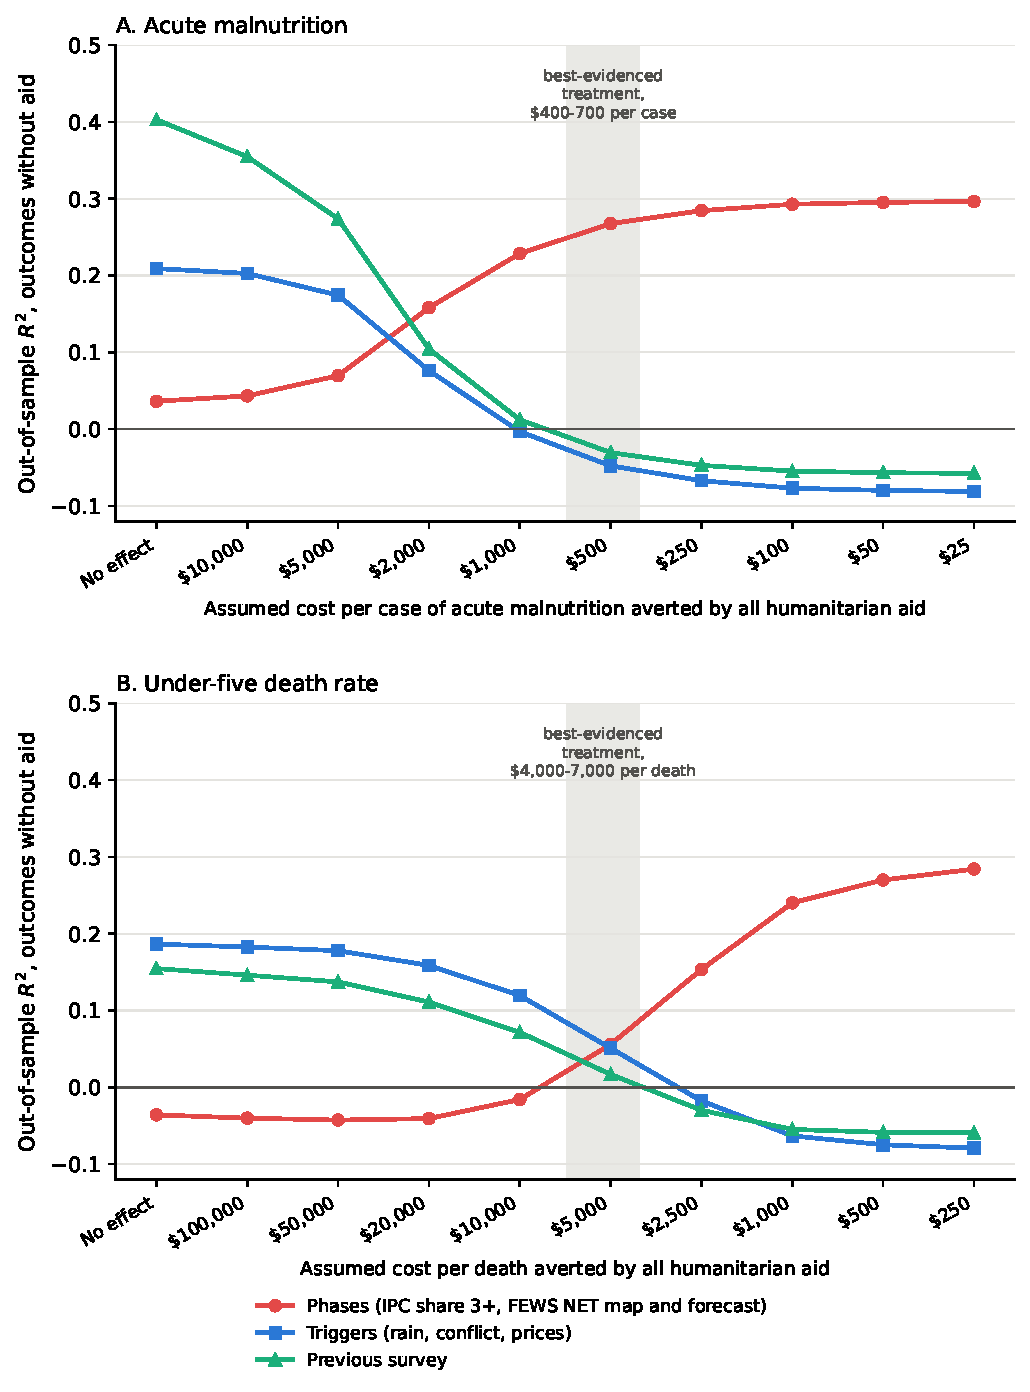
\includegraphics[width=0.95\textwidth,height=0.82\textheight,keepaspectratio]{figures/fig16_bounds.pdf}
\caption{Could aid be hiding the phases' value? Out-of-sample $R^2$ (equation~\ref{eq:predict}) for outcomes without aid (equation~\ref{eq:bounds}), Somalia's survey domains, by information set, as the assumed effectiveness of humanitarian aid rises (left to right). Panel A: acute malnutrition, against the assumed cost per case averted. Panel B: under-five death rate, against the assumed cost per death averted. Aid is assumed to be all humanitarian funding reported for Somalia (about \$\bdNatPc{} per person per six months), allocated in proportion to the IPC Phase 3+ share --- the allocation most favorable to the phases --- with half of averted deaths among children under five and ten cases of acute malnutrition averted per death. Shaded: community treatment of severe acute malnutrition, the best-evidenced life-saving intervention in crises, at \$4,000--7,000 per death averted (\$400--700 per case on the same assumption).}\label{fig:bounds}
\end{figure}

\paragraph{What would surveys be worth?} For surveys to save lives, a chain must hold: surveys give better information about where children are malnourished and dying; that information reaches the response; the response moves to where it is needed; and it saves lives there. The first link is strong, as above. The last is strong for treatment: treating severe acute malnutrition in the community averts a death for roughly \$4,000--7,000 on GiveWell's inputs for two well-run programmes \citep{givewell2024cmam,givewell2024taimaka}. The middle links are the weak ones. Survey results reach nutrition programmes directly, since programmes size their caseloads from measured prevalence \citep{isanaka2021icf}, but how far donors follow is less clear \citep{olin2014sida}, and programmes reach a minority of cases; average coverage across 21 countries was 38 percent \citep{rogers2015coverage}.

So we ask the counterfactual directly. We model a planner in Somalia who each season has a fixed number of treatment places for malnourished children in the \voiZones{} rural zones FSNAU surveys, and spends them to avert as many deaths as possible given what it can see. Severe acute malnutrition, about \voiSamShare{} percent of cases, carries an untreated one-year mortality of about 10 percent, which treatment cuts by about 70 percent; moderate acute malnutrition carries about 4 percent, cut by about 40 percent \citep{givewell2024cmam}. The planner predicts each zone's caseload from the national average, from FEWS NET's forecast phase, or from the zone's previous survey, all out of sample, and sends places where it predicts the most deaths averted. Places sent where cases turn out fewer than predicted are stranded unless they can be moved.

\begin{figure}[t]
\centering
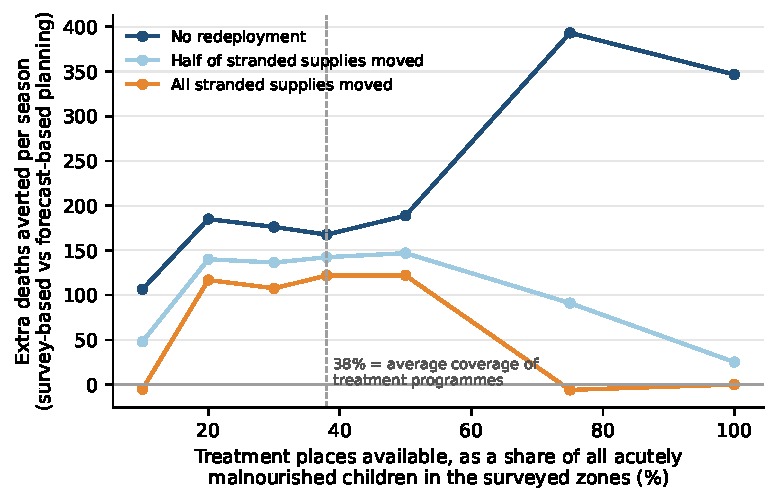
\includegraphics[width=0.72\textwidth]{figures/fig10_voi.pdf}
\caption{If treatment followed surveys: extra deaths averted per season in Somalia when a planner places treatment using each zone's previous scheduled survey rather than FEWS NET's forecast, by the size of the treatment budget: the number of treatment places as a share of all acutely malnourished children in the surveyed zones that season (horizontal axis). \voiZones{} surveyed rural zones per season over \voiSeasons{} seasons. The planner allocates treatment places to severe and moderate acute malnutrition by zone to maximize predicted deaths averted; places sent to zones with fewer cases than predicted are stranded, and none, half or all of them can be moved once caseloads are known. Mortality and treatment effects from GiveWell's inputs; caseloads from measured prevalence, population and the standard incidence correction.}\label{fig:voi}
\end{figure}

Survey-based planning saves more lives at every realistic budget (Figure~\ref{fig:voi}). With places for 38 percent of the caseload, a planner using FEWS NET's forecast averts about \voiBase{} deaths a season; one using the previous survey averts \voiGainFull{} to \voiGainZero{} more, depending on how many stranded places can be moved. That is \voiOracleZero{}--\voiOracleFull{} percent of the gain perfect foresight would bring. A planner who knows only population does about as well as one using the forecast. Most of the value comes from knowing where severe cases are. A round of surveys in these zones costs about \$\svvRound{} \citep{unicef_aah2016smart,daher2018smart}, so the extra deaths averted cost about \$\voiCostZero{}--\voiCostFull{} each, and \$\voiRangeLo{}--\voiRangeHi{} across budgets of 20--50 percent of the caseload. That is in the range of the most cost-effective charities.

This is an upper bound in one sense and a lower bound in another. It assumes treatment follows survey results as well as it could, which is the point of the exercise, not current practice. But it values surveys only for placing treatment within a fixed budget. It gives no credit for sizing the budget, for seeing famine-level conditions directly, for directing health, water and vaccination responses, or for knowing afterwards whether a response worked \citep{kenny2026humanitarian}.

\section{Where surveys do not go}\label{sec:gaps}

Surveys measure outcomes well only where they are run. Somalia's scheduled programme itself has often skipped insecure zones of the south --- Juba, South Gedo, parts of Bakool and Hiran --- or assessed them only by arm-circumference screening. In FEWS NET's reports, a survey from the previous 12 months is quoted for \svEmergET{} percent of areas mapped in Emergency in Ethiopia, \svEmergSO{} percent in Somalia and \svEmergSD{} percent in Sudan.

The pattern is general. We assembled metadata for every DHS, MICS and World Bank LSMS household survey in \gapCountries{} low- and middle-income countries from \gapYearZero{} to \gapYearOne{}. Across countries, surveys go where poverty is: their frequency falls steadily with income. Within a country over time, they avoid bad years. With country and year effects, a year of minor conflict lowers the chance that a survey starts by \gapAnyMinor{} percentage points (standard error \gapAnyMinorSe{}), and a year of war by \gapAnyWar{} (\gapAnyWarSe{}), from a base of \gapBase{} percent; a fall of more than 2 percent in GDP per capita lowers it by \gapAnyDown{} (\gapAnyDownSe{}). Around \gapOnsets{} conflict onsets, the chance of a survey drops by about \gapOnsetDrop{} points in the year a conflict starts and recovers within two years. The response comes mostly from the DHS; MICS surveys show no significant response to either conflict or downturns. Using five-year periods, \citet{trommlerova2026disease} find conflict a consistent negative predictor of whether a DHS or MICS takes place at all, with economic factors much weaker.

When surveys do go to conflict-affected countries, they often leave out the worst areas. We coded the sampling appendices of \exReports{} DHS and MICS reports from 2000 on, covering every survey run in a country with recent battle deaths and a random sample from calm countries. Some area or selected cluster was dropped for insecurity or inaccessibility in \exCalm{} percent of reports from calm countries, \exMinor{} percent under minor conflict and \exWar{} percent in wartime (Figure~\ref{fig:exclusions}). In about one in five conflict-country surveys, whole districts or regions were cut from the design before fieldwork began: the north of Mali in 2012 and 2015, 20 of Borno's 27 local government areas in Nigeria's 2021 MICS, and five districts of Nainawa in Iraq's 2018 MICS, whose report nonetheless says its teams visited every selected area. \exCampsSilent{} percent of reports never mention camps; \exCampsOut{} explicitly exclude them and \exCampsIn{} include them, mostly in special designs for refugee populations. Only \exDisplQ{} of the questionnaires we coded identify displaced people.

\begin{figure}[t]
\centering
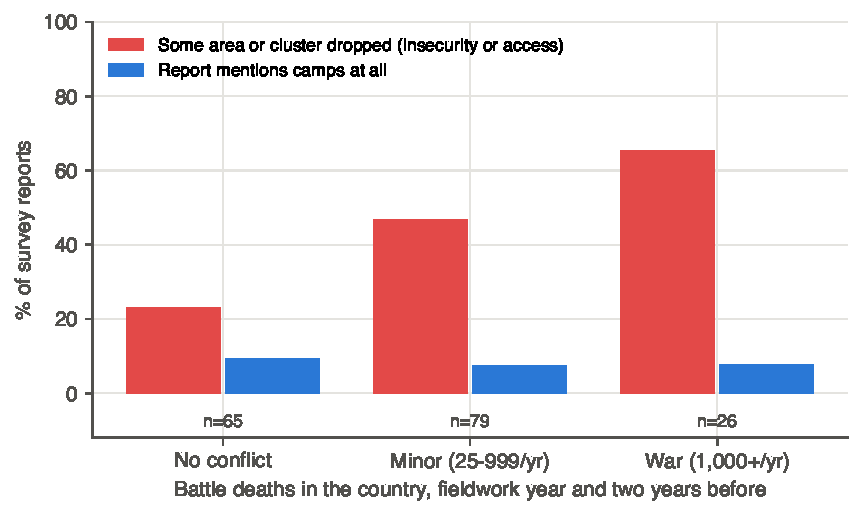
\includegraphics[width=0.72\textwidth]{figures/fig12_survey_exclusions.pdf}
\caption{What household surveys leave out. Share of DHS and MICS final reports (2000 onward) that document dropping an area or selected cluster for insecurity or inaccessibility (red), and that mention camps at all (blue), by battle deaths in the country in the fieldwork year and the two years before. \exReports{} reports with usable sampling text; coded from the reports' sampling appendices.}\label{fig:exclusions}
\end{figure}

This matters because the deaths are mostly outside camps. Across 1,759 death-rate estimates from crises between 1998 and 2012, refugees' death rates sat near their host baselines, while those of internally displaced people were 2.5 times baseline and residents' 1.5 times \citep{heudtlass2016}; the burden has long been shifting to populations outside camps \citep{salama2004,spiegel2010}. These are general-purpose household surveys, not the nutrition surveys of Section~\ref{sec:surveys}, but the lesson carries over. A system that relies on surveys will see least where conditions are worst, unless it is designed for those places: scheduled rather than alarm-driven, with methods for insecure areas such as remote and phone-based data collection, community mortality surveillance and sampling of displaced people outside camps.

\section{Implications}\label{sec:implications}

Four changes follow from the evidence, in increasing order of ambition. They concern the IPC's scale and the way phase counts are used; FEWS NET forecasts that scale, and would follow it.
\begin{enumerate}
  \item \textbf{Stop converting phases into deaths.} The reference bands for malnutrition and mortality are not calibrated to phases, and measured gradients are a fraction of them. Estimates of lives at stake built by multiplying people in Crisis or worse by the bands overstate deaths in some crises and understate them in others. Death rates, where they matter for classification, should be read against local baselines \citep{deZwarte2026Lancet}.
  \item \textbf{Report outcomes next to phases.} Each IPC analysis could report the latest measured acute malnutrition and mortality for each area, with dates, and flag areas with none. That costs little and makes clear when a phase count rests on no outcome data at all.
  \item \textbf{Pay for scheduled surveys and surveillance in high-risk areas.} Somalia's scheduled rounds show what a fixed calendar buys: results that predict the next round and are not driven by where alarm happened to be raised. Our estimates put the value of such surveys, if treatment followed them, at about \$\voiRangeLo{}--\voiRangeHi{} per death averted. They would need to be designed for the places current surveys avoid --- insecure districts, displaced people outside camps --- using methods built for those settings.
  \item \textbf{Target downstream outcomes.} If most crisis deaths come from disease, a system that sizes and prioritizes crises by people in food insecurity directs attention to a small part of the problem. A response organized around forecasts of malnutrition and mortality would put more weight on measles vaccination, water and sanitation, malaria and diarrhoea treatment and therapeutic feeding --- the measures the public health literature has long found most effective --- and could save more lives with the same budget.
\end{enumerate}

The first two are technical changes the IPC partnership could make. The last two would change what the humanitarian system optimizes, and they raise questions we cannot settle here. Mortality is harder and more dangerous to measure than food consumption, especially where conflict is worst. Concentrating on deaths wherever they occur, rather than on the camps and sites that are easiest to reach and measure, is right in principle but would shift resources toward places that are hard to serve. And food insecurity is a harm in itself, not only a route to death; a system that stopped counting it would lose something. These are arguments for testing the larger proposal against the views of practitioners, not for dismissing it.

\FloatBarrier
\appendix
\section{Method}\label{app:method}

For a survey of area $a$ in season $t$, with measured outcome $y_{at}$ (acute malnutrition, or a crude or under-five death rate) and FEWS NET phase $P_{at}$ (its forecast for the survey month, or its map), we estimate
\begin{equation*}
y_{at} = \beta P_{at} + \mu_a + \lambda_t + \varepsilon_{at}.
\end{equation*}
Without the area effects $\mu_a$, $\beta$ compares different areas: are areas in worse phases worse off? With them, it compares the same area over time: when an area is one phase worse than usual, how much worse are its outcomes? The season effects $\lambda_t$ remove shocks common to the country in a season. We also score FEWS NET's forecast as a predictor of $y_{at}$ out of sample, leaving out one season at a time, against the simplest alternative: the area's own measurement in the previous round.

\paragraph{Somalia.} We kept FSNAU's rural SMART surveys and matched each surveyed zone to FEWS NET's mapping units by livelihood zone and region. Mean acute malnutrition was \fsGam{} percent, and \fsCrit{} percent of zone-seasons were at or above the critical level of 15 percent. FEWS NET's forecast was issued a median of \fsLead{} months ahead of the survey. FSNAU's analysts work alongside FEWS NET's, though the survey measurements are independent of the classifications.

\paragraph{Household indicators.} Areas are matched to FEWS NET's map for the same month by averaging the phase over the FEWS NET units in the survey area. The IPC thresholds used for the 20 percent rule are those of the IPC reference table: borderline food consumption at Crisis, poor at Emergency or worse, and a reduced coping strategies index of 19 or more at Crisis or worse.

\paragraph{Survey timing.} The country-year panel covers \gapCountries{} countries, \gapYearZero{}--\gapYearOne{}. The outcome is whether fieldwork for a DHS (including malaria and AIDS indicator surveys), a MICS or an LSMS started in the year. Conflict is battle deaths from the Uppsala Conflict Data Program, as published in the World Development Indicators (minor conflict: 25--999 deaths; war: 1,000 or more). Linear probability models with country and year effects; standard errors clustered by country. For DHS alone the effects are \gapDhsMinor{} (\gapDhsMinorSe{}) points for minor conflict, \gapDhsWar{} (\gapDhsWarSe{}) for war and \gapDhsDown{} (\gapDhsDownSe{}) for a downturn, from a base of \gapBaseDhs{} percent.

\paragraph{Survey exclusions.} Reports were downloaded from the DHS Program, the World Bank and IHSN microdata catalogs and IPUMS-MICS. Sampling passages were extracted automatically and coded by a language model against a fixed codebook (areas excluded at the design stage, clusters dropped in the field and why, camps excluded or included, displacement questions), with spot checks against the text. Silence is coded as ``not mentioned'', not as ``not excluded''.

\begin{figure}[H]
\centering
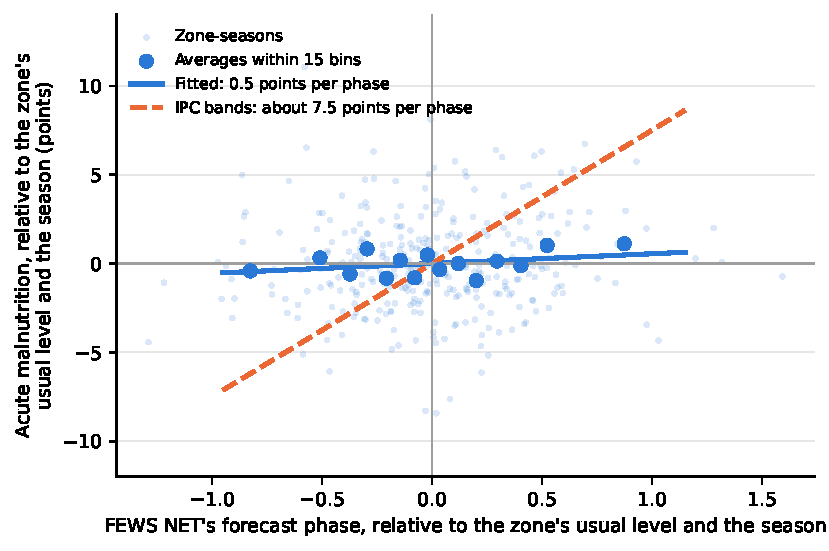
\includegraphics[width=0.82\textwidth]{figures/fig9c_within_zone.pdf}
\caption{Within zones: when FEWS NET forecasts a Somali zone to be worse than usual, is its measured malnutrition worse than usual? Both variables are measured relative to the zone's own average and the season's average across zones. Light points: \fsN{} zone-seasons; dark points: averages within 15 equal-sized bins of the forecast. Solid line: fitted slope. Dashed line: the slope implied by the IPC reference bands, roughly the average of the 5- and 10-point steps between band midpoints.}\label{fig:within}
\end{figure}

\begin{figure}[H]
\centering
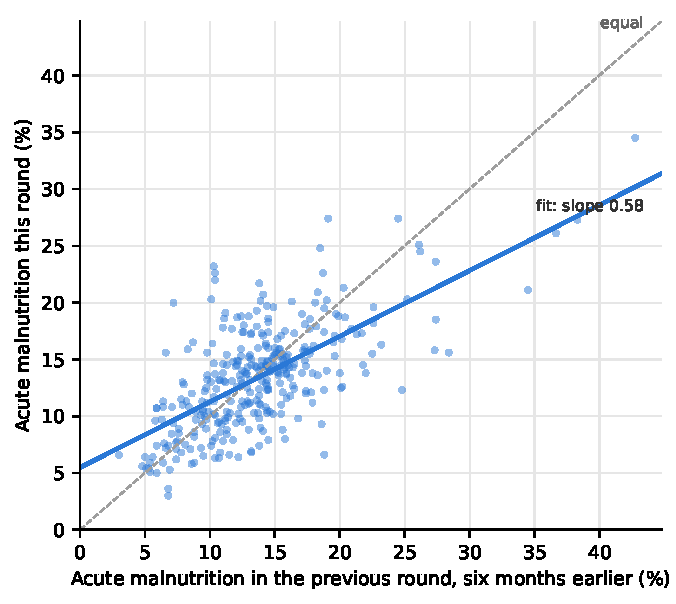
\includegraphics[width=0.62\textwidth]{figures/fig9d_persistence.pdf}
\caption{Somalia's scheduled surveys: acute malnutrition in a rural zone this round against the same zone six months earlier, \fsN{} zone-seasons, 2011--2024. Solid line: least-squares fit; dashed line: equality.}\label{fig:persist}
\end{figure}

\begin{figure}[H]
\centering
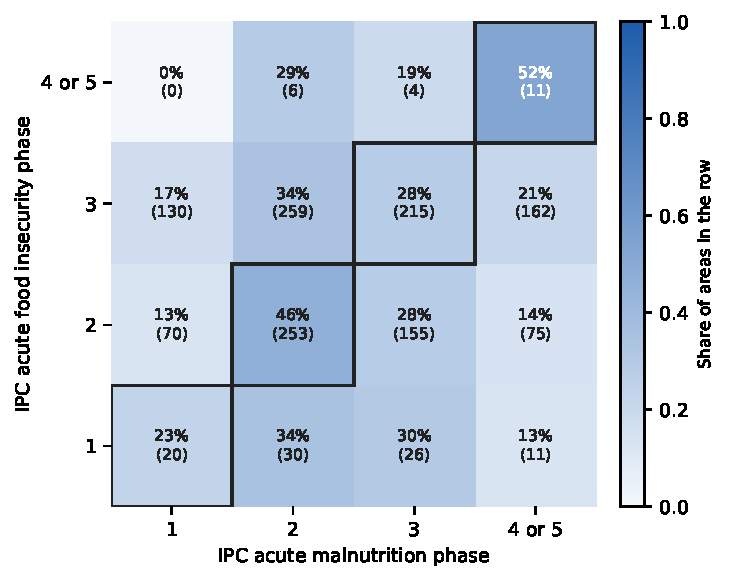
\includegraphics[width=0.66\textwidth]{figures/fig9e_afi_amn.pdf}
\caption{The IPC's two scales for the same areas. Rows: the IPC acute food insecurity phase of the area; columns: its acute malnutrition phase for the same period (published by the IPC, or classified from published acute malnutrition prevalence using the IPC's thresholds). Each cell gives the share of the row and the number of areas; outlined cells are where the two scales agree. \amnAnyN{} areas in Afghanistan, the Central African Republic, Cameroon, the Democratic Republic of Congo, Mali, Mozambique, Nigeria, Somalia and South Sudan, 2021--2026 (years vary by country).}\label{fig:amn}
\end{figure}

\newpage
\bibliographystyle{chicago}
\bibliography{references}
\end{document}
